\documentclass[12pt]{article}
\title{China -- The Empire That Did Not Bark \footnote{following the Sherlock Holmes story ``Silver Blaze'' by Sir Arthur Conan Doyle, Holmes was able to deduce that the killer of Colonel Ross's racehorse was the owner of the stable dog, the dog that did not bark. What does not happen is often as important as what does.}\\
}
\author{Stephen C. Bannister\\
	Department of Economics\\
	343 Orson Spencer Hall\\
	University of Utah\\
	Salt Lake City, Utah 84112\\
	USA\\
	\href{mailto:steve.bannister@econ.utah.edu}{steve.bannister@econ.utah.edu}\\
	}
%\date{\today}
\date{}
\usepackage[latin1]{inputenc}
\usepackage{amsmath}
\usepackage{mathtools}
\usepackage{amsfonts}
\usepackage{txfonts}
\usepackage{amssymb}
%\usepackage{amsthm}
\usepackage{pgfpages}
\usepackage{booktabs}
\usepackage{longtable}
\usepackage{verbatim}
\usepackage[justification=centering]{caption}
\usepackage{hyperref}

\usepackage{natbib}
\bibpunct{(}{)}{;}{a}{,}{,}
%\usepackage{glossaries}
\linespread{2.0}	% remove for single, 1.3 for 1.5 and 1.6 for 2.0. use this setting for print editing

\newtheorem{mydef}{Definition}[section]
\numberwithin{equation}{section}

\begin{document}

\raggedright

\graphicspath{{../images/}}
%\graphicspath{{../images_pub/}}

%\bibliographystyle{plain}
	\maketitle

\newpage
	China -- The Empire That Did Not Bark\\
	\begin{abstract}
	Recent scholarship demonstrates that late imperial China and early modern Europe were broadly similar in terms of economic possibilities, yet then experienced radically different growth trajectories.
	
	I argue that this divergence, the English Industrial Revolution, had primarily fortuitous geographic and economic, rather than cultural or institutional, causes. China did not undergo the underlying energy revolution that England did because it did not have necessary \textit{economic} conditions, although it had sufficient institutions.
	\end{abstract}
	\section*{Introduction and research questions}
	While there are sufficient unsettled questions for a career, here I focus on those key facts about China and its paradoxical failure to participate in the growth miracle emerging from the English Industrial Revolution.
	
	Given that recent scholarship suggests that eighteenth-century per-capita incomes in England and similar parts of China were roughly comparable and had both grown somewhat since the sixteenth century, why did English output then accelerate into the first continually sustained period of per-capita growth ever experienced and Chinese output, at least relatively, stagnate? 
	
	China, a highly integrated society sharing world population dominance with India, by all the known rules explaining economic dynamics up to that time as summarized by the Reverend Thomas Malthus, should have dominated the world economy. And it did. From Angus Maddison's data (\citeyear{maddison_maddison_2010}), China and India had roughly 50 percent of both world population and gross domestic product (GDP) at the beginning of the sixteenth century, while England accounted for 1 percent of population and 1 percent of GDP. Yet England's growth so dominated the eighteenth and nineteenth century that in $1900$ England's share of world GDP was 9 percent while her population was only 3 percent of the world total. China and India's combined share of GDP in $1900$ had fallen to 20 percent while their combined population was still 44 percent of the world total. %\footnote{\citet{maddison_maddison_2010}}
	
	Many scholars search for and discern some combination of social, cultural, and/or institutional factors to explain the phenomenon of the Industrial Revolution. Yet the magnitude of the post eighteenth-century growth trajectory differences imply a level of English exceptionalism in those factors that strains credulity. Are we to believe that, over a very few generations, English ``growth enabling'' institutions somehow grew sufficiently superior to Chinese to account for the growth differences? This class of explanation is even more problematic in that it at least implicitly assumes that some one or some group understood what institutions were needed for this sui generis event and had the power to form them.
	
	A further mystery is the ``Needham question,'' that arises from the fact, as Joseph Needham (\citeyear{needham_science_1954}) documented in the seven volumes of ``Science and Civilisation in China,'' that China had great scientific and technological discoveries but lost the ``race'' to both the Scientific and Industrial Revolutions. This supports the idea of functionally sufficient Chinese institutions of the very kind needed to supply the inventions required to participate in the revolutions.
	
	Further, in the long sweep of history, England had a relatively brief period of per-capita growth dominance. By no later than 1875, the growth revolution was quickly spreading to North Western Europe, North America, and Meiji Japan. If England's lead in growth was uniquely determined by a specific set of exceptional institutions, is there evidence that such usually long-gestation changes in culture, institutions, and society itself were so quickly transmitted to other cultures?
	
	And if transmitted institutional exceptionalism accounts for the rapid spread of growth, why was it transmitted relatively narrowly until the second half of the twentieth century? Why didn't China immediately converge? Is the relevant effect in fact that societies oppose fundamental economic changes that in turn cause societal changes until the economic forces becoming overwhelming? Was China ``not barking'' because there was nothing to bark at, because the dog saw nothing but the long familiar non-threatening agrarian empire? This explanation is certainly consistent with a story of China not enjoying English-style exceptionalism. Or, is it rather a story that there were no Chinese economic forces that at the macro level would have driven Chinese entrepreneurs to English style energy innovation. The literature on English exceptionalism, from Weber through Landes to McCloskey is well known; I focus elsewhere.
	
	In this paper I explore the counter question: what underlying \textit{economic} reasons might account for this remarkable series of events and non-events? I argue elsewhere that what England discovered and transmitted, initially  narrowly, to the world, was an energy revolution in economic activity. Why did China fail to follow that revolutionary path until the twentieth century? Does \textit{economics} provide a more satisfactory explanation \ldots within the simplifying context of Ockham's Razor \ldots than "exceptionalism?"
	
	The question is one of primary causality, not monocausality. Institutionalists claim that superior institutions were the primary cause of the Industrial Revolution. I claim that superior economic conditions were the primary cause, while fully acknowledging as proximate the supporting and surrounding institutional and cultural fabric.	
	
	\section*{Contribution}
	Stipulating that institutions in regions of China and in England had produced essentially the same standard of living by $1800$, and that the market systems were roughly equivalent, I present a story of the \textit{energy revolution} that China did not experience (and that England did). The differences, explained by different macro and micro market forces, and geological and geographical luck, are not only sufficient to explain the divergence in their post-$1800$ economic paths, but, I argue in detail elsewhere, were the necessary conditions for the English Industrial Revolution to occur. China missed a microeconomic incentive that England enjoyed, and therefore also missed the macroeconomic network effects of a virtuous feedback cycle that became the Industrial Revolution. 
	
	I use comparative descriptions and empirics to demonstrate that English economic factors and geographical luck created a \textit{energy} revolution that substituted fossil energy for organic sources as the prime mover for the Industrial Revolution. This replaces arguments for English institutional exceptionalism as the prime mover. China, with a brief historical exception, did not experience a fossil energy revolution \textit{because} their economic fundamentals did not support it.
	
	Extending Robert Allen's (\citeyear{allen_british_2009}) high-wage theory of the English Industrial Revolution, I formalize the microeconomic (factor-price substitution) argument, apply it to China, and demonstrate \textit{why} at the micro level the Chinese had no energy revolution and therefore no Industrial Revolution. 
	
	I make the background macroeconomic argument explicit only here in this paper: Chinese wages levels must have been insufficient to generate income levels supporting robust effective demand for market-provided consumer goods. At the micro (incentive) level, this implies the derived marginal revenue product (demand) curve for labour was relatively shifted left, reinforcing low wage levels in those product markets. Chinese inventors thus had no economic incentive to commercialize their inventions capable of substituting relatively more expensive (in China) fossil energy for relatively less expensive human energy.
	
	\section*{Comparative historical data and observations}
	
		For context, to understand the scale of the divergence, I begin by examining world population, gross domestic product, and the resultant per-capita GDP through the current historical period, covering the crucial pre-industrial and Industrial Revolution periods, and showing the current levels for context. The initial data is from Maddison (\citeyear{maddison_maddison_2010}). Maddison measures GDP in 1990 International Geary-Khamis Dollars, that describe purchasing power parity (PPP) adjusted output. Maddison's data set, whatever its challenges, is widely cited and is where many comparative scholars start. I also start with it. 

\begin{center}		
Figure \ref{fig:poplevel1900} about here		
\end{center}
 				
		The top two panels of figure \ref{fig:poplevel1900} show that both world population and GDP levels for years CE 1500 through 1900 underwent unprecedented growth; the bottom two proportion panels demonstrate that much of the growth was in Europe and the western offshoots. It is clear that China and India dominated both world population and GDP until about $1700$. After that, when world GDP started a period of super-exponential growth, the proportion charts show that Western Europe and the United States dominated GDP growth, and had population growth above the world rate.
		
		The pattern of faster population growth rate in both Chinese and English proto-industrial periods, though on this chart the English growth is hard to see, remains an open demographic question (Kenneth Pomeranz \citeyear[p.~22]{pomeranz_great_2001}).  \footnote{One theory (Alfred Crosby and others) asserts that the post-``Columbian Exchange'' arrival in Europe and China of American crops like maize and potatoes increase agricultural productivity per land unit by 3 or 4 times, enabling a rise in otherwise Malthusian subsistence population levels.  (Alfred Crosby \citeyear{crosby_columbian_1972})} To abstract from that I next examine per-capita GDP growth.
		
		\subsection*{Comparative per-capita GDP}			

\begin{center}		
Figure \ref{fig:capita} about here		
\end{center}

		Figure \ref{fig:capita} shows per-capita GDP by regional and national groupings of interest from CE 1 through 1900, using the underlying Maddison (\citeyear{maddison_maddison_2010}) data. Here, two facts stand out. First, China maintains a relatively constant level of per-capita GDP throughout the period. China did not become absolutely poorer; however, China did not share in the great average output growth of the Western nations. Second, the grouping I denote the EU-11, \footnote{The EU-11 grouping includes Austria, Belgium, Denmark, Finland, France, Germany, Italy, the Netherlands, Norway, Sweden, and Switzerland.} led by England, is increasing in per-capita GDP starting in $1500$, with rapid increases after $1800$. The Western Offshoots show a similar growth pattern of per-capita GDP. The sustained productivity growth arising during the Industrial Revolution led to sustained standard-of-living increases. This sui generis episode of modern economic growth stands in stark contrast to China and the rest of the world. \footnote{The Western Offshoots are statistically dominated by the United States, but also include Canada, Australia, and New Zealand.}
		
		The lack of a growth pattern in Chinese per-capita GDP leads to a fascinating question: How much is our perception of this fact coloured by our twenty-first century point-of-view? More formally, what would our expectations for the rate of growth of per-capita GDP have been as an astute economic observer in eighteenth-century China? Or, for that matter, in England?
		
		The evidence is that the classical economists had no expectations for any prolonged positive growth in GDP per-capita because they had never observed that phenomenon. Thomas Malthus clearly represents the then widespread point-of-view that expectations were for subsistence GDP, essentially zero-growth per capita levels forever. Thus our fascination with what actually happened, and our dramatically different modern expectations.
		
\begin{comment}		
		
		The next several charts illuminate these dramatic changes.

	
		\begin{figure}[htb]
		\centering
		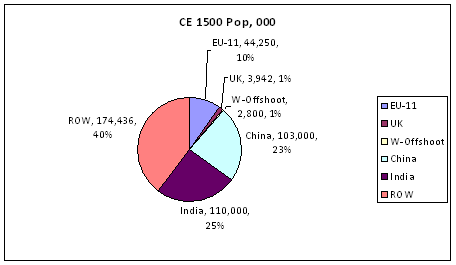
\includegraphics[width=0.8\textwidth]{1500pop.png}
		\caption{World population shares, 1500 CE}
		\label{fig:1500pop}
		\end{figure}
			
		\begin{figure}[htb]
		\centering
		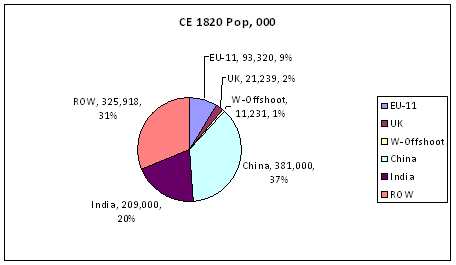
\includegraphics[width=0.8\textwidth]{1820pop.png}
		\caption{World population shares, 1820 CE}
		\label{fig:1820pop}
		\end{figure}
		
		\begin{figure}[htb]
		\centering
		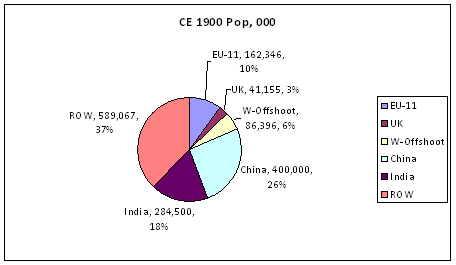
\includegraphics[width=0.8\textwidth]{1900pop.png}
		\caption{World population shares, 1900 CE}
		\label{fig:1900pop}
		\end{figure}
		
		Figures \ref{fig:1500pop}, \ref{fig:1820pop}, and \ref{fig:1900pop} trace the evolution of global population shares from CE $1500$ through $1900$ grouped by major regions. We see China undergoing a population explosion and collapse between CE $1500$ and $1900$, with a peak share of $37\%$ of world population in $1820$. England is on a steady growth march, starting at $1\%$ share in $1500$ and ending at $3\%$ in 1900. We can perhaps discern the proto-industrial population growth in both economies prior to $1820$, and only England continues growth after that that.
		
%		\newpage
		
		\begin{figure}[htb]
		\centering
		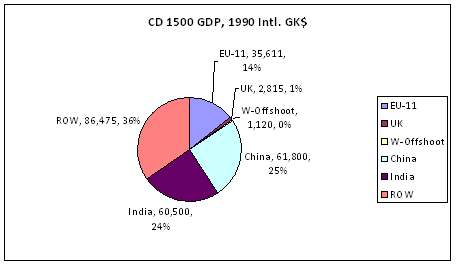
\includegraphics[width=0.8\textwidth]{1500gdp.png}
		\caption{World GDP shares, 1500 CE}
		\label{fig:1500gdp}
		\end{figure}
		
		\begin{figure}[htb]
		\centering
		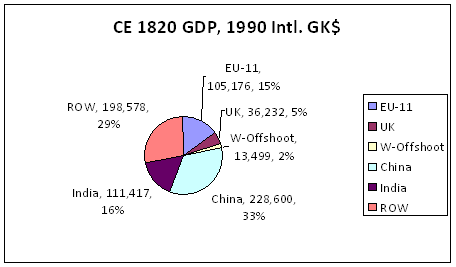
\includegraphics[width=0.8\textwidth]{1820gdp.png}
		\caption{World GDP shares, 1820 CE}
		\label{fig:1820gdp}
		\end{figure}
		
		\begin{figure}[htb]
		\centering
		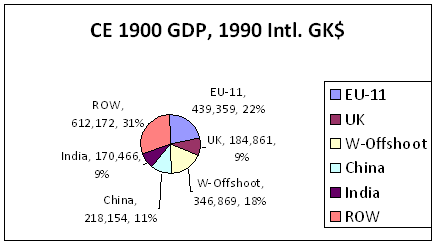
\includegraphics[width=0.8\textwidth]{1900gdp.png}
		\caption{World GDP shares, 1900 CE}
		\label{fig:1900gdp}
		\end{figure}
		
		Figures \ref{fig:1500gdp}, \ref{fig:1820gdp}, and \ref{fig:1900gdp} trace the path of global GDP shares from CE $1500$ through $1900$ grouped by major regions. We see China's gobal GDP share staying roughly in line with its populations share, so peaking in $1820$ at the end of the world proto-industrial era.
		
		England's GDP share has grown dramatically, from the $1\%$ proportional to its population share in $1500$, to $2.5$ times population share in $1820$, to $3$ times population share in $1900$.
		
\end{comment}
		
		These charts represent highly aggregated numbers, and thus potentially mask important underlying structural and regional differences, especially in China. Kenneth Pomeranz, for example, asserts that the standard of living in regions of China was equivalent to Western Europe in $1800$ (differently than the Maddison data that, however, is for all of China), and that the standard of living wage levels in the Lower Yangzi region in China were at English levels in $1800$ (Pomeranz \citeyear[p.~107]{pomeranz_great_2001}). Decomposing the standard of living into wages and cost-of-subsistence softens those differences except in the Lower Yangzi, but in any case we need to explain the post-$1820$ divergence.
		
		Two main explanatory threads oppose each other: One thread appeals to institutional differences, the other to economic and geographic differences exploited by inventor/entrepreneurs. The essential factor to decode is the \textit{prime} mover, recognizing that there are interaction effects over time that are surely important.
		
		I question the institutional argument that the prime mover in the Industrial Revolution was English institutional exceptionalism, and set up the economic/geographical prime mover hypothesis; this suggests analyzing the growth divergence between China and England as an exercise in comparative micro- and macroeconomics. But first I examine the political economies to establish the essential institutional sufficiency for growth in each country.
%to here
		\newpage

		\subsection*{Comparative Political Economies }
		
		The logic for rejecting institutional exceptionalism as prime is that whatever the institutional differences between China and England, there were sufficient similarities to yield similar economic results up until $1800$ at least in the most comparable Chinese region, the Lower Yangzi. It is thus difficult to imagine sufficient institutional differences to cause such a dramatic divergence over the next century. This logic appeals to the work of R. Bin Wong and Kenneth Pomeranz.
		
		First, comparative political economies in post-$1500$ late Imperial China and early modern Europe from R. Bin Wong:
		
		\begin{quotation}
		
		``The Chinese state maintained an active interest in the agrarian economy, promoting is expansion over large stretches of territory and its stability through uneven harvest seasons\ldots Despite considerable variation in techniques, there was basic agreement through the eighteenth century about the type of economy officials sought to stabilize and expand. They supported an agrarian economy in which commerce had an important role'' (R. Bin Wong \citeyear[pp.~115--16]{wong_china_1997}).
		\end{quotation}
		
		\begin{quotation}
		``Mercantilism, the dominant philosophy of political economy in Europe between the late sixteenth and the early eighteenth century, posed a close relationship between power and wealth. For a state to become powerful, society had to become wealthier. This was achieved by expanding economic production in rich core areas and by extending trade across the country and especially beyond it\ldots competition for wealth on a global scale became a component of European state making. European states promoted the production and commerce of their private entrepreneurs, whose successes contributed to the consolidation and prosperity of competing states'' (Wong \citeyear[p.~140]{wong_china_1997}).
		
		\end{quotation}
		
		Wong thus contrasts a Chinese imperial agrarian state interested in social stability with a group of European power elites competing over a zero-sum economic game with military Mercantilism. Yet, until the eighteenth-century divergence, roughly the same level of subsistence was the norm.

		
		Moving to Kenneth Pomeranz who evaluates Chinese and English, Asian and Western European, economic levels at more granular scales involving agriculture, transport, and livestock capital, longevity, health and nutrition, birthrates, accumulation, and technology.
		
		\begin{quotation}
		``\ldots as late as the mid-eighteenth century, western Europe was not uniquely productive or economically efficient\ldots many other parts of the Old World were just as prosperous and ``proto-industrial'' or ``proto-capitalist'' as western Europe\ldots What seems likely is that no part of the world was necessarily headed for such a [industrial] breakthrough.''
		
		``\ldots the production of food, fiber, fuel, and building supplies all competed for increasingly scarce land\ldots western Europe\ldots became a fortunate freak only when unexpected and significant discontinuities in the late eighteenth and especially nineteenth centuries enabled it to break through the fundamental constraints of energy use and resource availability that had previously limited \textit{everyone's} horizons\dots the new energy itself came largely from a surge in the extraction and use of English coal\ldots'' (Pomeranz \citeyear[pp.~206--07]{pomeranz_great_2001})
		\end{quotation} 
		
		Pomeranz's detailed comparative evaluation thus somewhat contradicts Maddison's data, and highlights both institutional differences and similarities, but the differences are irrelevant in the end simply because England uniquely led the organic to fossil energy transition that was the revolutionary foundation for, and the prime mover at the center of, the Industrial Revolution. I next turn to the economic incentives that England had, and China did not, to make that transition.
		
		
\begin{comment}		
		\subsection{Comparative internal markets}
			\subsubsection{England}
			high wages, high food prices, equal income distribution, growing consumer demand, land intensive vs. labour intensive agriculture, a pre-industrial pattern, deforestation, cheap accessible coal.
			\subsubsection{China}
			low wages, low food costs, labour intensive agriculture, a pre-industrial pattern, deforestation, expensive inaccessible coal.
		\subsection{Comparative external markets}
			\subsubsection{England}
			\subsubsection{China}
\end{comment}
			
		\subsection*{The Road to Riches}
		
		About which I argue causally involved microeconomic incentives creating emergent macro effects in a self-reinforcing positive feedback loop. Thus, what are possible economic explanations as prime movers of the Industrial Revolution since the evidence for causal institutional exceptionalism appears insufficient?
		
		There are at least two, one microeconomic and factor substitution driven, and one macroeconomic. \footnote{We can proceed either with a neo-classical factor substitution argument, or a more general classical view of normal prices of production. Either approach will react to the enormous productivity-enhancing energy supply shock that was the Industrial Revolution. A more challenging story to tell is one which identifies the sources of aggregate demand that supported expansion of English production. Here, I simply stipulate that aggregate demand existed.}
		
		Robert Allen proposes a relatively simple factor substitution argument that relies on differences in relative labour and energy prices between China and England, most dramatically between Newcastle and the rest of the world. Essential to his argument is that England, almost uniquely, was a high wage economy (Allen \citeyear[p.~34]{allen_british_2009}). This is illuminated in figure \ref{fig:allen_wages}. 
		
\begin{center}
Figure \ref{fig:allen_wages} about here
\end{center}		
		
		He also examines world energy prices, which I do not reproduce here, although England had the lowest energy prices in the world. This led to a high English wages-to-energy prices ratio that fuelled the energy transition, notably so compared to China (Allen \citeyear[p.~140]{allen_british_2009}). The basis for this argument can be seen in the next figure. 

\begin{center}
Figure \ref{fig:allen_ratios} about here
\end{center}			
		
		
		Figure \ref{fig:allen_ratios} shows that the relative price ratio of wages to energy prices was highest in Newcastle and lowest in Beijing. Thus, there was a strong economic incentive to substitute coal energy for human energy in Newcastle and almost none in Beijing. This microeconomic effect is founded on London heating demand and, with the spread of high wages, increasing demand for market-supplied consumer goods.
		
		The effect of Allen's graph can be explained using basic microeconomic theory. If an entrepreneur has two substitutable sources of energy inputs, say human and coal, her profit maximizing behaviour is described as in the following equation where the Marginal Revenue Product is the amount of revenue generated by the last joule input to the production process:
		\begin{equation}
		\label{mrp}
		\frac{\text{Marginal Revenue Product}_{\text{ organic energy joule}}}{\text{Price}_{\text{ organic energy joule}}} = \frac{\text{Marginal Revenue Product}_{\text{ fossil energy joule}}}{\text{Price}_{\text{ fossil energy joule}}}
		\end{equation}
		
		Assume that the production technology is neutral on the source of joules, i.e. an $\text{ organic energy joule}$ is equal in marginal revenue product to a $\text{fossil energy joule}$. Then if the price of fossil energy is sufficiently lower than the price of organic energy, as in the case of England, she will substitute coal for humans until the price of human energy equals the price of coal energy, which is probably never. Refer to equation \ref{mrp}. That condition did not exist in China, so the micro-incentive never kicked in.
		
		Allen further argues the following logic chain: Coal was plentiful and cheap in both Northwest and Northeast England. As London grew rapidly due to English success in international trade, London experienced high wages that spread throughout England, and faced increasing heating prices due to local deforestation. Thus, beginning in the sixteenth century, the ``coal-burning house'' that was invented in London led English coal demand and production to increase (Allen \citeyear[p.~82]{allen_british_2009}).  See figure \ref{fig:allen_coal}.
		
\begin{center}
Figure \ref{fig:allen_coal} about here
\end{center}
		


		English coal mines had an important geological problem with water infiltration; human or animal pumping became increasingly expensive and lacked scale as coal demand increased and the mines went deeper. The first real, practical use of the inefficiently crude Newcomen steam engines was to pump the water from the mines using otherwise surplus coal. As the inventions became more efficient, they became both the literal and figurative engines of the Industrial Revolution (Allen \citeyear[pp.~86 -- 93]{allen_british_2009}).
		
		Kenneth Pomeranz tells a different story, an essentially macro story. Beyond his revisionist and contested view of eighteenth century China and England being at essentially similar development levels, he contends that Western Europe was running out of land, was thus at the precipice of impending land scarcity (Allen \citeyear[p.~264]{allen_british_2009}). Pomeranz further contends the English ``escape'' was due to coal and colonies. To illustrate the growth dilemma I prepared the chart in figure  \ref{fig:eng_wood}. 
		
\begin{center}
Figure \ref{fig:eng_wood} about here
\end{center}
			

	
		Figure \ref{fig:eng_wood} is the result of a counterfactual exercise asking if it was feasible for England to meet its actual energy consumption demand during the Industrial Revolution by substituting other energy sources for coal -- in this particular experiment wood.  The graph shows that England would indeed have required \textit{all} of its landmass to be forest in order to supply a sustainable fuel source to meet its energy requirements by the last quarter of the nineteenth century (Roger Fouquet \citeyear{fouquet_heat_2008}). England ``escaped'' this bottleneck by learning how highly scalable fossil-energy based macroeconomies are. The graph for the Chinese counterfactual experiment, using recent energy consumption data, shows a similar pattern, and a remarkably similar outcome -- China is now approaching the point at which the entire country would be forested if it had to provide its energy demand with wood.
		
		To illustrate how powerful the virtuous feed-back cycle was from English entrepreneurs individually substituting coal for humans, figure \ref{fig:mtoe_log} is a log of English energy consumption, showing the structural breaks and related change in slopes. The slope changes in this chart indicate a super-exponential growth in energy consumption, a signature of the English energy revolution.

\begin{center}
Figure \ref{fig:mtoe_log} about here
\end{center}
			
				
		Pomeranz further provides a macroeconomic story of the lack of a sustained mineral energy transition in China. What is stunning from his telling is that eleventh-century Song China \textit{did} start a coal-based energy transition. It was based on the large coal and iron deposits in North and Northwest China close to the then political, demographic, and economic center. Chinese iron production in $1080$ likely exceeded non-Russian European production in $1700$ (Pomeranz \citeyear[p.~62]{pomeranz_great_2001}).
		
		The region was then subjected to a series of ``staggering catastrophes'' (Pomeranz \citeyear[p.~62]{pomeranz_great_2001}) including Mongol invasions and occupations, civil wars, enormous floods, and plague. The demographic and economic centers shifted south, incurring large transportation costs for raw materials. Coal-based industrialization never recovered until well into the twentieth century despite eighteenth century attempts by the government to develop the mines to alleviate fuel shortages in the Lower Yangzi Delta.
		
		Further, while this is an intriguing historical event, there is no evidence that the Chinese had any path-dependent incentives to develop steam engines as the technical problem in the Chinese coalfields was (and is) ventilation to prevent spontaneous combustion, not the water pumping problem of English fields. And thus they did not develop industrial steam engines.
		
\begin{comment}
			\subsubsection{England}
			\subsubsection{China}
		\subsection{What did they expect?}
		
		\subsection{the cottrell theory}
			
	\section{Literature Review}
	Karl Marx\\
	Fred Cottrel\\
	R. Bin Wong\\
	\section{Discussion}
\end{comment}

	\section*{The empirical energy evidence}
	
	In other work related to my dissertation, I use English energy consumption time series dating to CE $1300$ and establish a strong correlation over history between energy consumption and GDP.
	
	Chinese historical energy data remains elusive, though my search continues. What follows is data from Angus Maddison and others, that is at least suggestive (Maddison \citeyear[p.~10]{maddison_growth_2003}).
	
	Maddison, in a 2003 paper, publishes a table titled ``Primary Energy Consumption Per Capita, Major Countries, 1820 -- 1998.'' The units are metric tonnes of oil equivalent consumed per capita. I have extended his table into Table \ref{tab:maddison_energy} that summarizes the relevant data.

\begin{center}
Table \ref{tab:maddison_energy} about here
\end{center}	

	
	Energy consumption is the central theme in my theory of development, growth, and the Industrial Revolution. Chinese per- capita energy consumption in 1973 was $79\%$ of English consumption in 1820, and only $22\%$ of English consumption in 1870.
	
	Also, during those 50 years, the peak of the English Industrial Revolution, English per-capita energy consumption increased by a factor of 3.6. 
	
	Vaclav Smil notes the following:
	
	\begin{quotation}
	``By 1700 typical levels of energy use, and hence of material affluence, were still broadly similar in China and Western Europe. Then the Western advances gathered speed \ldots By 1850 the two societies belonged to two different worlds. By 1900 they were separated by an enormous performance gap: Western European energy use was at least four times the Chinese mean'' (Vaclav Smil \citeyear[p.~234]{smil_energy_1994}).
	\end{quotation} 
	
	China, in the late twentieth century, finally started down what I hypothesize as the \textit{only} path to development, by following its own energy consumption revolution.
	
	\section*{Conclusion}

	China failed make a permanent transition from organic energy to fossil mineral energy until 150 years after the English Industrial Revolution. The failure is not surprising given no other civilization made the transition until the English and especially so considering the great luck in economics, geography, and geology the English enjoyed that supported their revolution. China did not enjoy that luck, except fleetingly. This was not an institutional failure.
	
	Economically, England enjoyed success in international trade that caused a growing and high-wage London population to deforest her environs and demand consumer goods. This created a demand for the cheap coal from the north to heat London and begin to substitute for high-wage labour in industrial production.
	
	Geographically, the north east had tidewater coal, so was close to the cheapest bulk transport of the time, the sea. Also, the northwest had iron deposits, thus co-locating the ore and fuel required to produce iron in an economically advantageous physical juxtaposition. 
	
	Geologically, the English coal fields were water infiltrated, leading to the invention, starting with Newcomen, of ever more efficient coal-fired steam engines capable of pumping deep water and powering the Industrial Revolution. These replaced high wage English labour in English factories and thus created an industrial scale far beyond anything wood, human or, animal power was capable of. The engines also became the foundation of the nineteenth-century railroad- and steamship-driven transportation revolution.
	
	These three fortunate juxtaposed events caused the Industrial Revolution, the great transition in food, fuel, fiber, and building materials that determined the economic future of the world. China enjoyed no such fortunes.
	
	China, ironically, experienced an early coal-fired iron revolution that never had the opportunity to develop into a sustained energy transition due to the bad luck of two centuries of ``staggering catastrophes.'' The economic and demographic center shifted away from the resource-advantaged region, and the industry did not recover. China did not subsequently experience the economic drivers of high wages and cheap energy.
	
	Further, China's mine geology did not have the paradoxically favorable water-infused conditions that led to English steam-power engine superiority.
	
	Yet, China's fleeting early eleventh-century energy transition success suggests that geographical luck is prime in the Industrial Revolution, not institutional exceptionalism. Functionally the same institutions that existed then existed in the eighteenth and nineteenth centuries when China failed to make the transition with different geo-spatial economic conditions.
	
	The empirical evidence on energy consumption, sparse though it currently is, strongly suggests a Chinese economy that failed to make the energy transition crucial to modern development until late in the twentieth century.

\begin{comment}	
	\section{Appendix - Imperial Chinese Dynasties}
	
%	\begin{table}
%	\centering
%	\caption{Chinese Imperial Dynasties}
	\begin{tabular}{ll}
	Empire&Historical Era\\
	\hline \hline
	Qin Dynasty &221--206 BC\\
	Han Dynasty &202 BC--AD 220\\
	Wei and Jin Period &AD 265--420\\
	Wu Hu Period &AD 304--439\\
	Southern and Northern Dynasties &AD 420--589\\
	Sui Dynasty &AD 589--618\\
	Tang Dynasty &AD 618--907\\
	Five Dynasties and Ten Kingdoms &AD 907--960\\
	Song, Liao, Jin, and Western Xia Dynasties &AD 960--1234\\
	Yuan Dynasty &AD 1271--1368\\
	Ming Dynasty &AD 1368--1644\\
	Qing Dynasty &AD 1644--1911\\
	\hline
	\end{tabular}
%	\label{tab:chin_dyn}
%	\end{table}
	
\end{comment}
	
	\newpage
	\section*{References}
%	\bibliographystyle{E:/LaTeX-Portable/MikTex-Portable/bibtex/bst/base/plain-annote}
	\bibliographystyle{agsm}	
		\bibliography{empire}
		
\newpage
\section*{Tables}

\begin{table}[htb]
	\centering
	

	\begin{tabular}{lrrrr}
	\hline
	Year&England&China&Netherlands&India\\
	\hline \hline
	1650$^a$&&&0.63&  \\
	1820&0.61&&&\\
	1840$^a$ &&&0.33& \\
	1870&2.21&\\
	1970$^a$ &&&8.07&0.33 \\
	1973&&0.48&&\\
	1998$^b$&6.56&1.18\\
	2008$^b$&5.99&2.56&9.86&  \\
	\hline
	\end{tabular}
	\caption{Per-Capita Primary Energy Consumption,	annual Tonnes of Oil Equivalent. \textit{Source:} Angus Maddison, $^a$de Zeeuw, $^b$US DOE EIA}
	\label{tab:maddison_energy}

	\end{table}



\newpage
\section*{Figures}

		\begin{figure}[]
		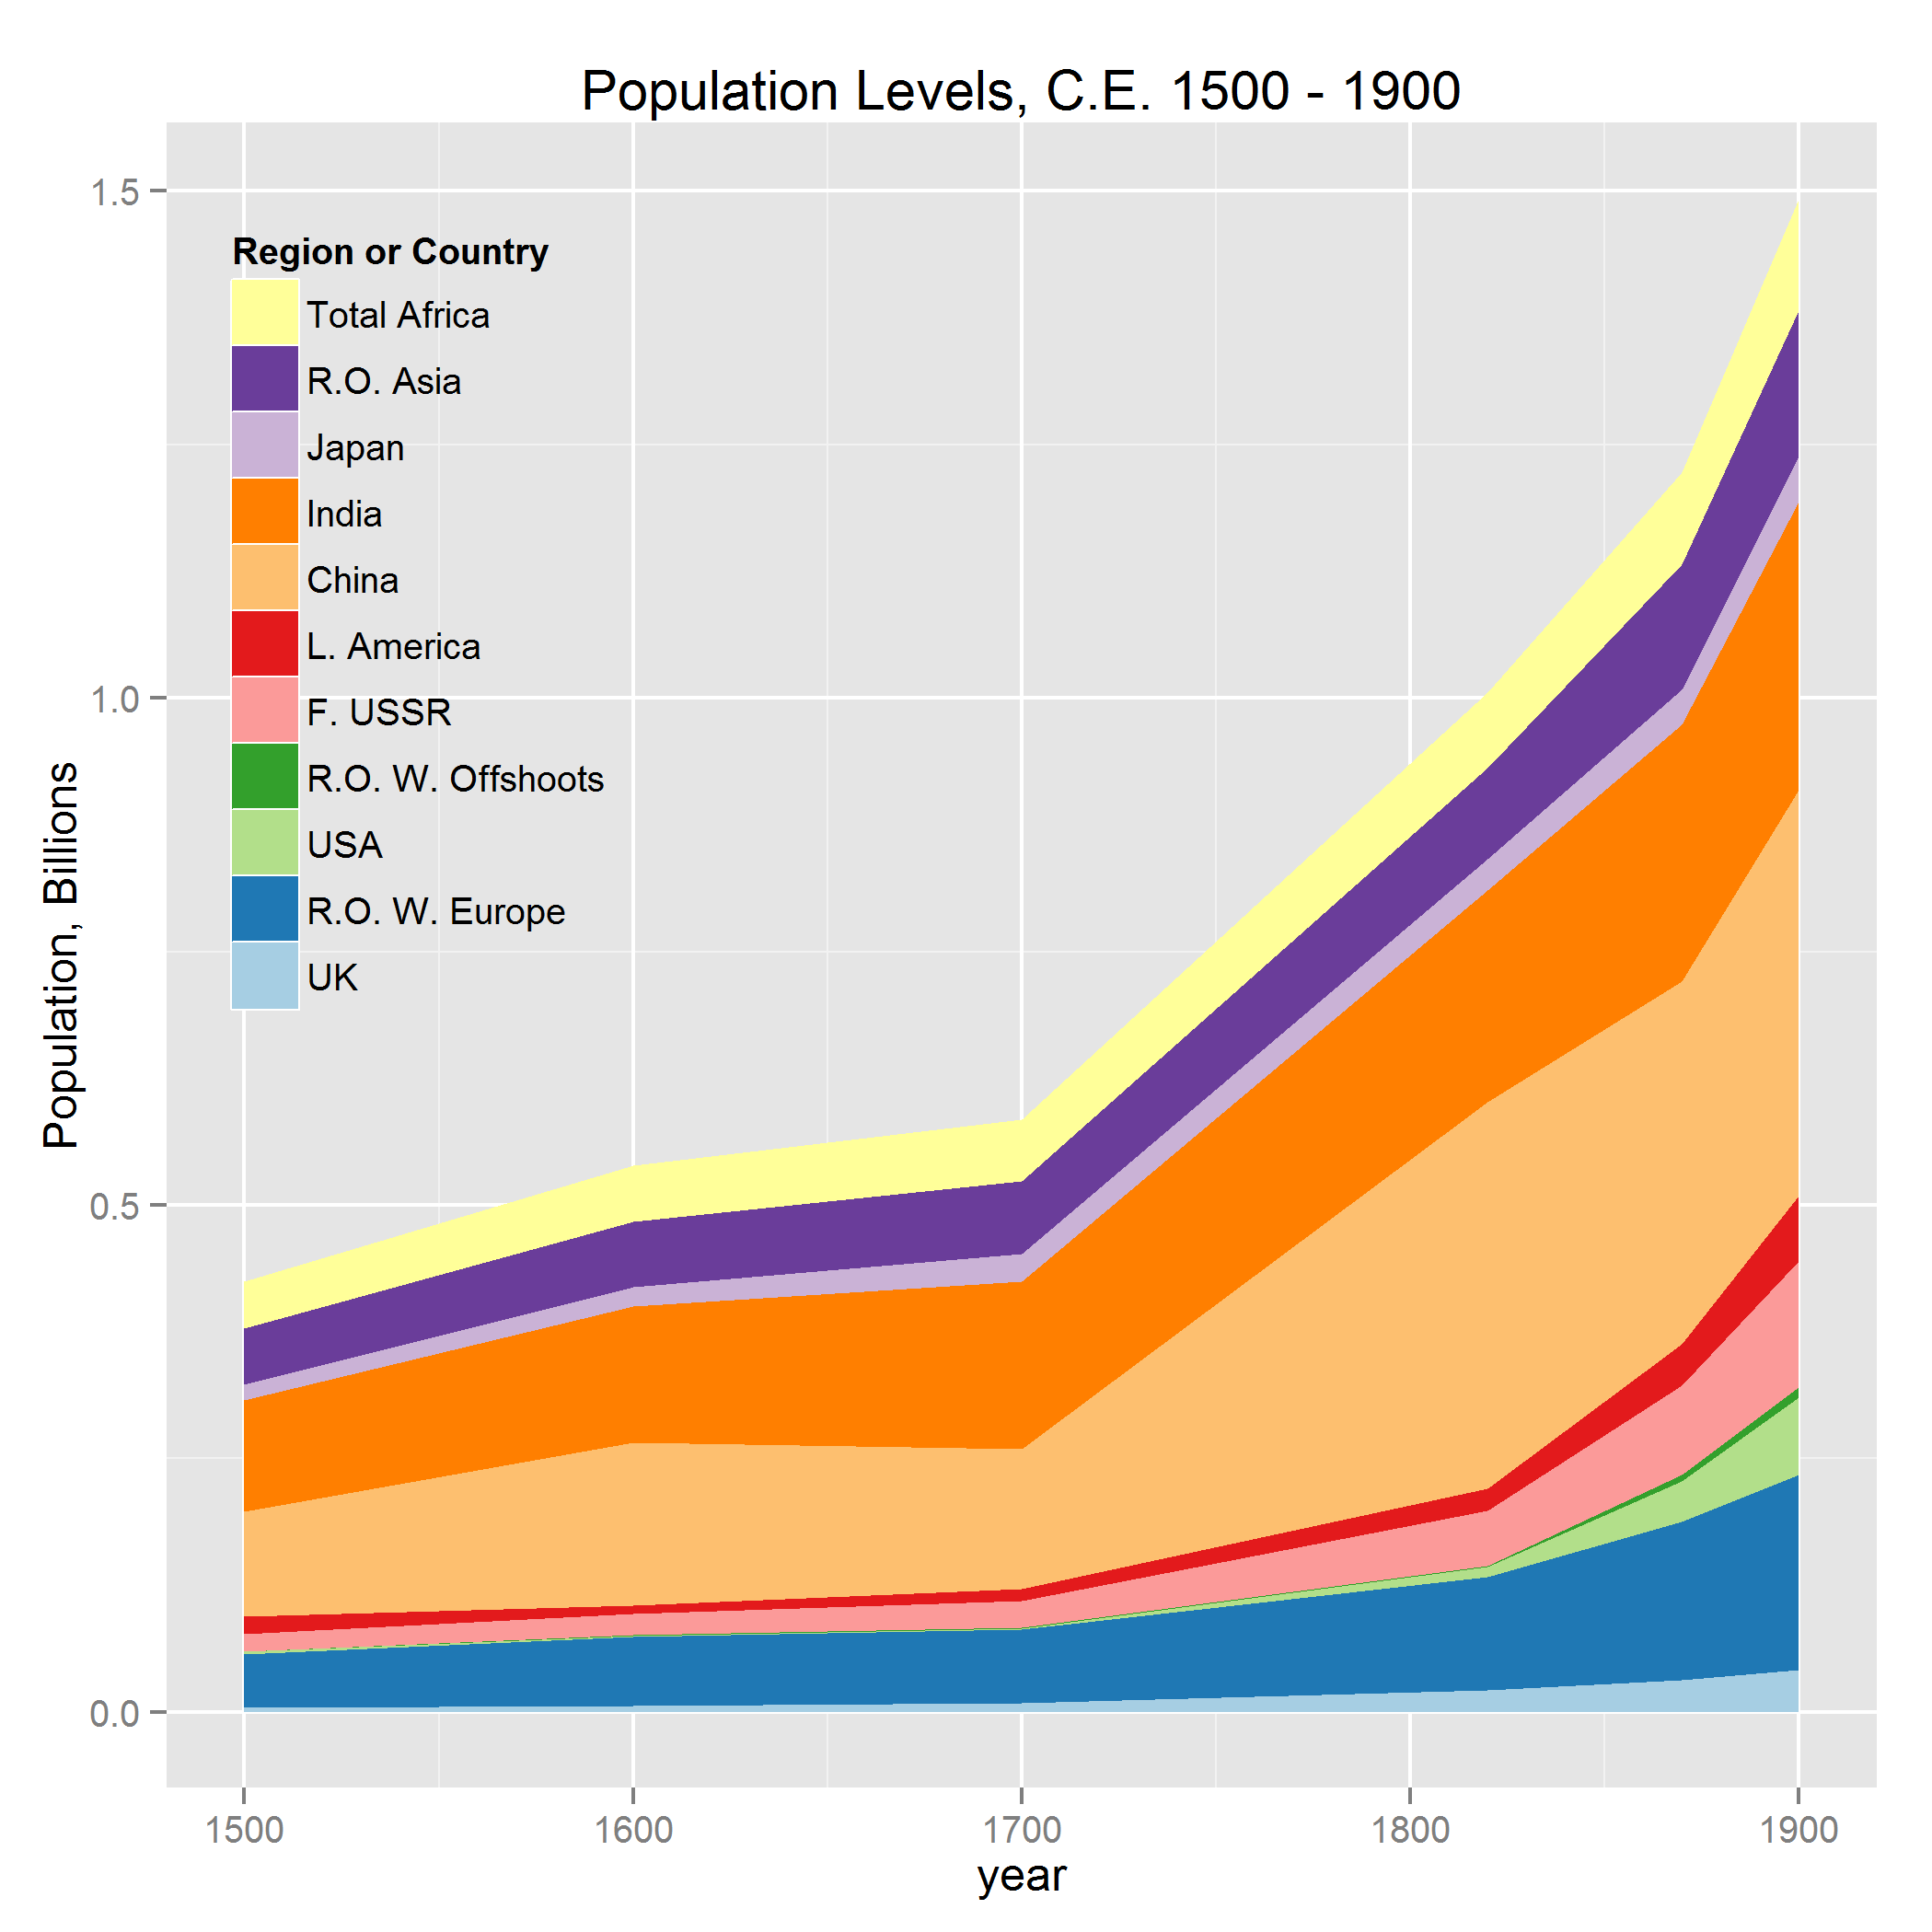
\includegraphics[width=0.5\textwidth]{maddisonregpoplevels1900.png}
		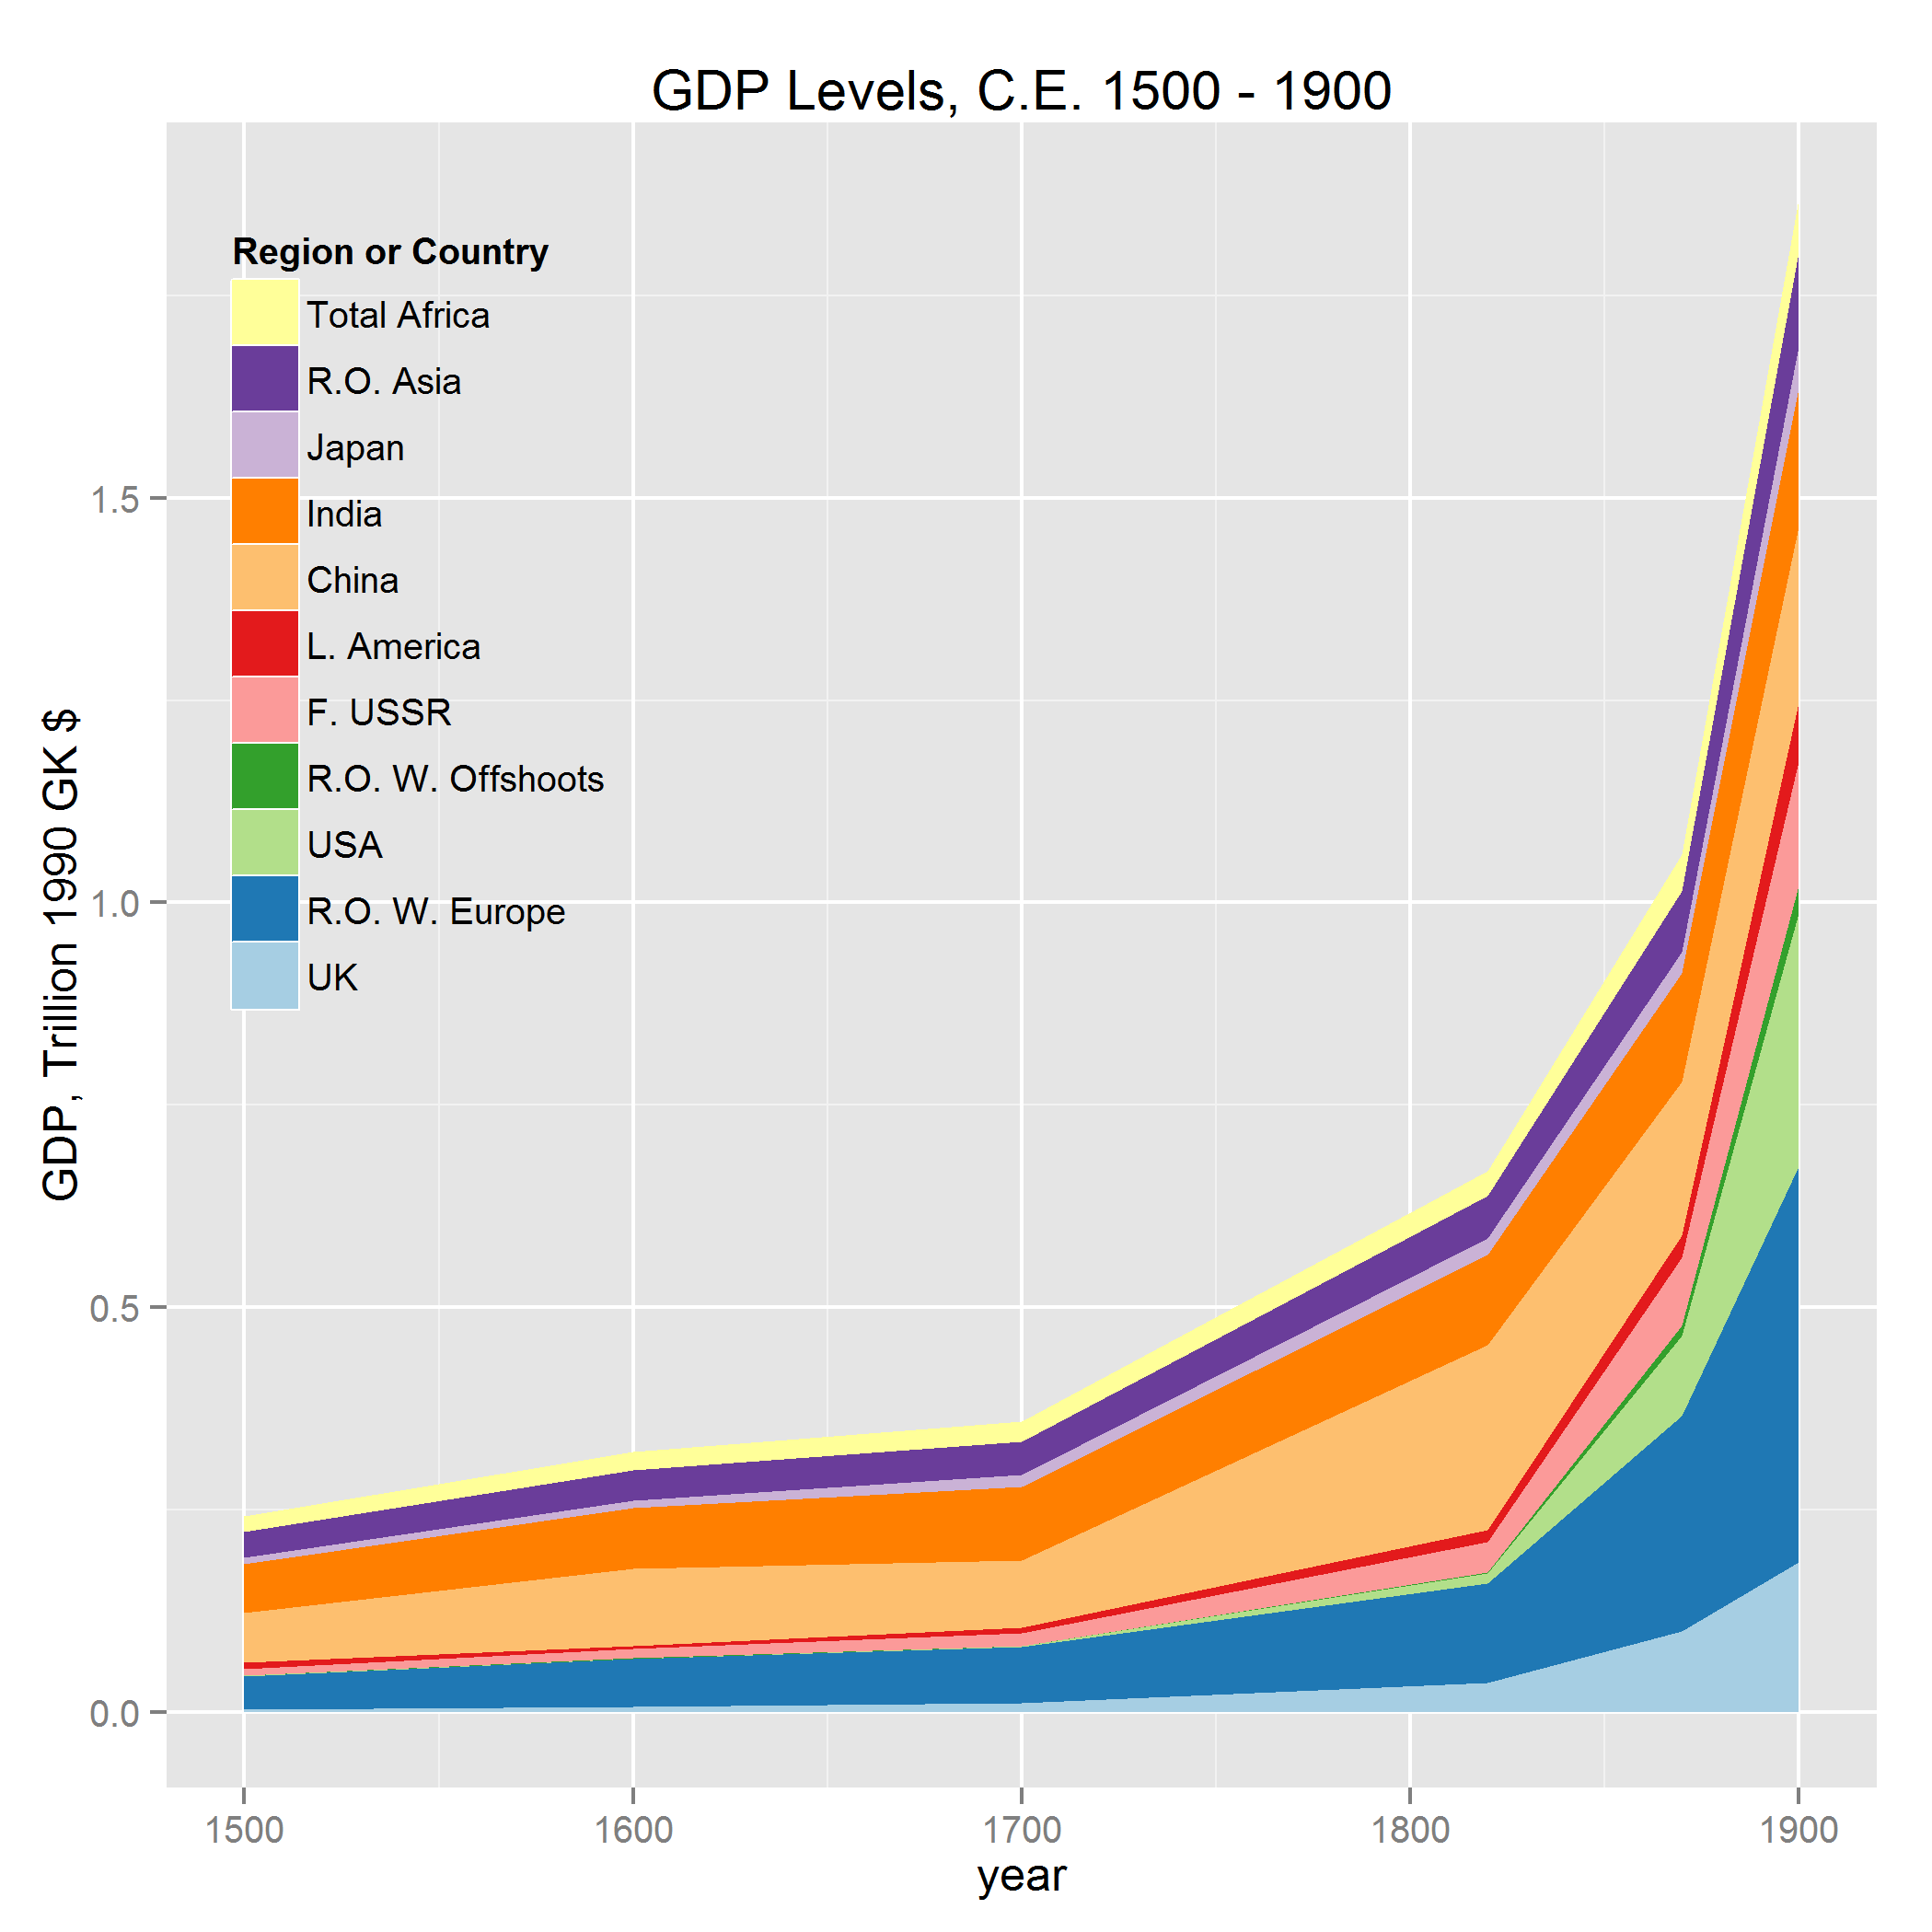
\includegraphics[width=0.5\textwidth]{maddisonreggdplevels1900.png}\\
		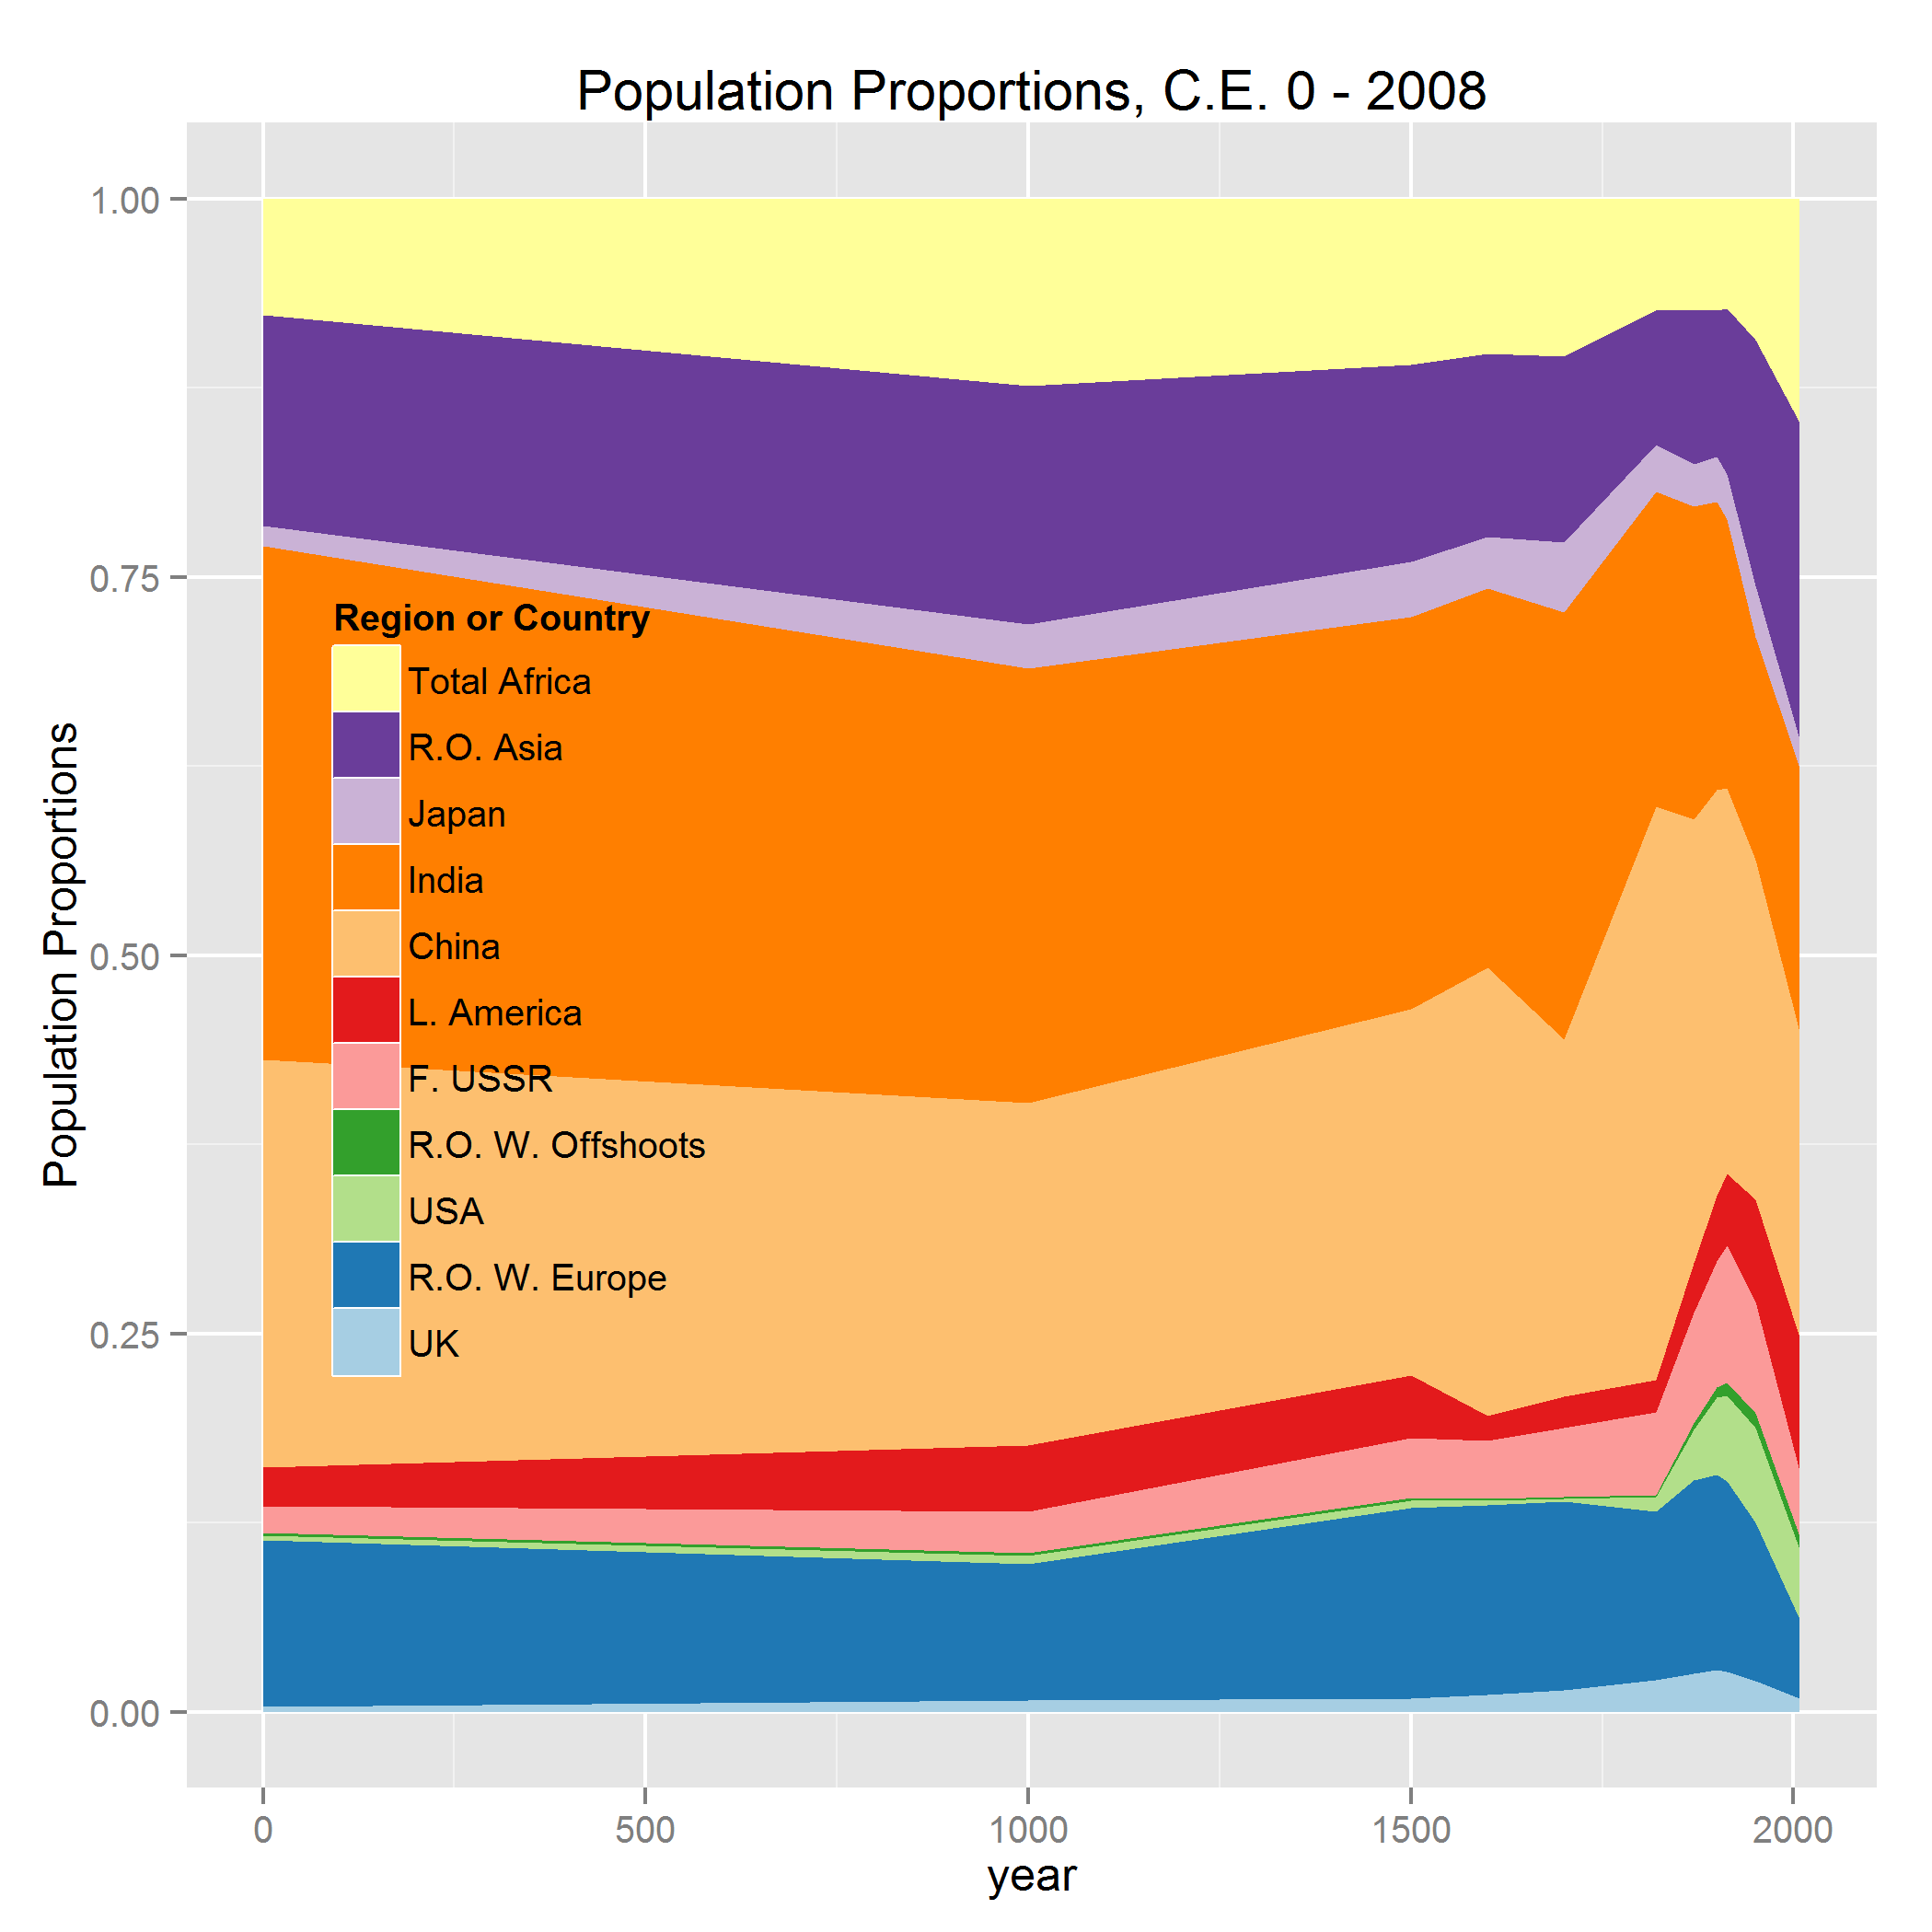
\includegraphics[width=0.5\textwidth]{maddisonregpoppct.png}
		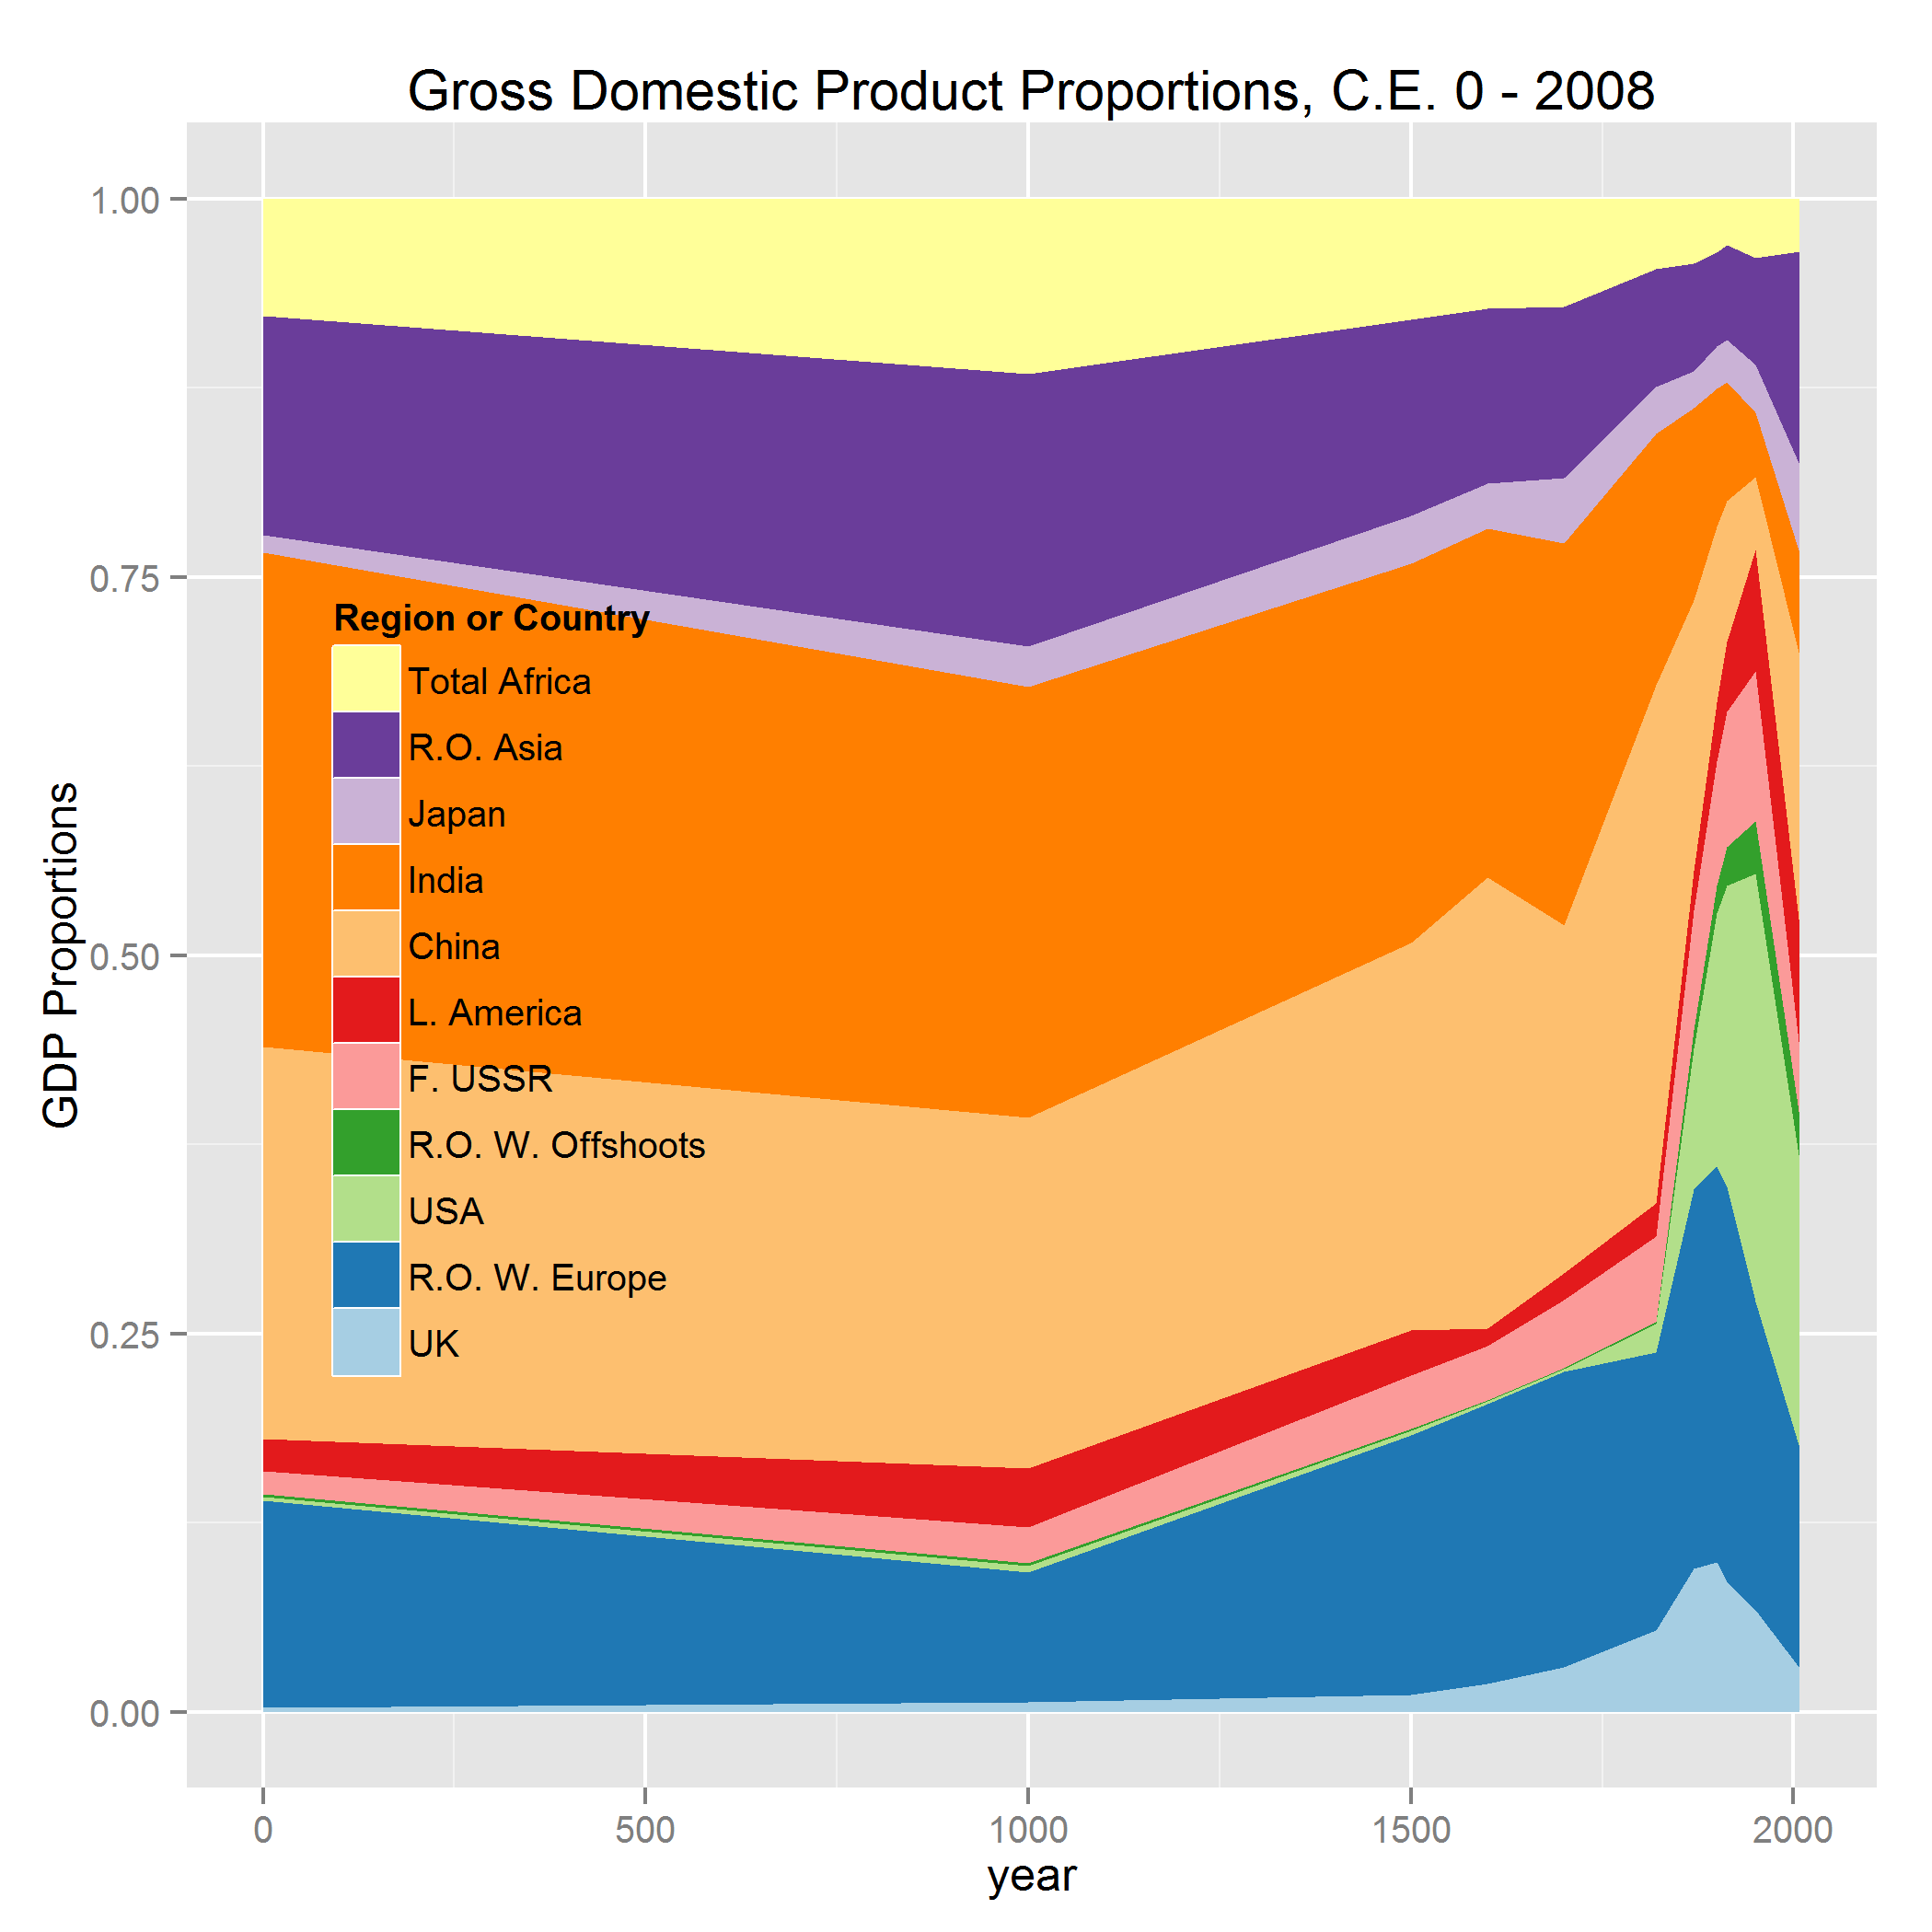
\includegraphics[width=0.5\textwidth]{maddisonreggdppct.png}
		\caption{Population and GDP levels from 1500 to 1900; population and GDP proportions from 0 to 2008. \textit{Source:} Data from Maddison (\citeyear{maddison_maddison_2010}), graphs by author.}
		\label{fig:poplevel1900}
		\end{figure}	
		
		\begin{figure}[]
		\centering
		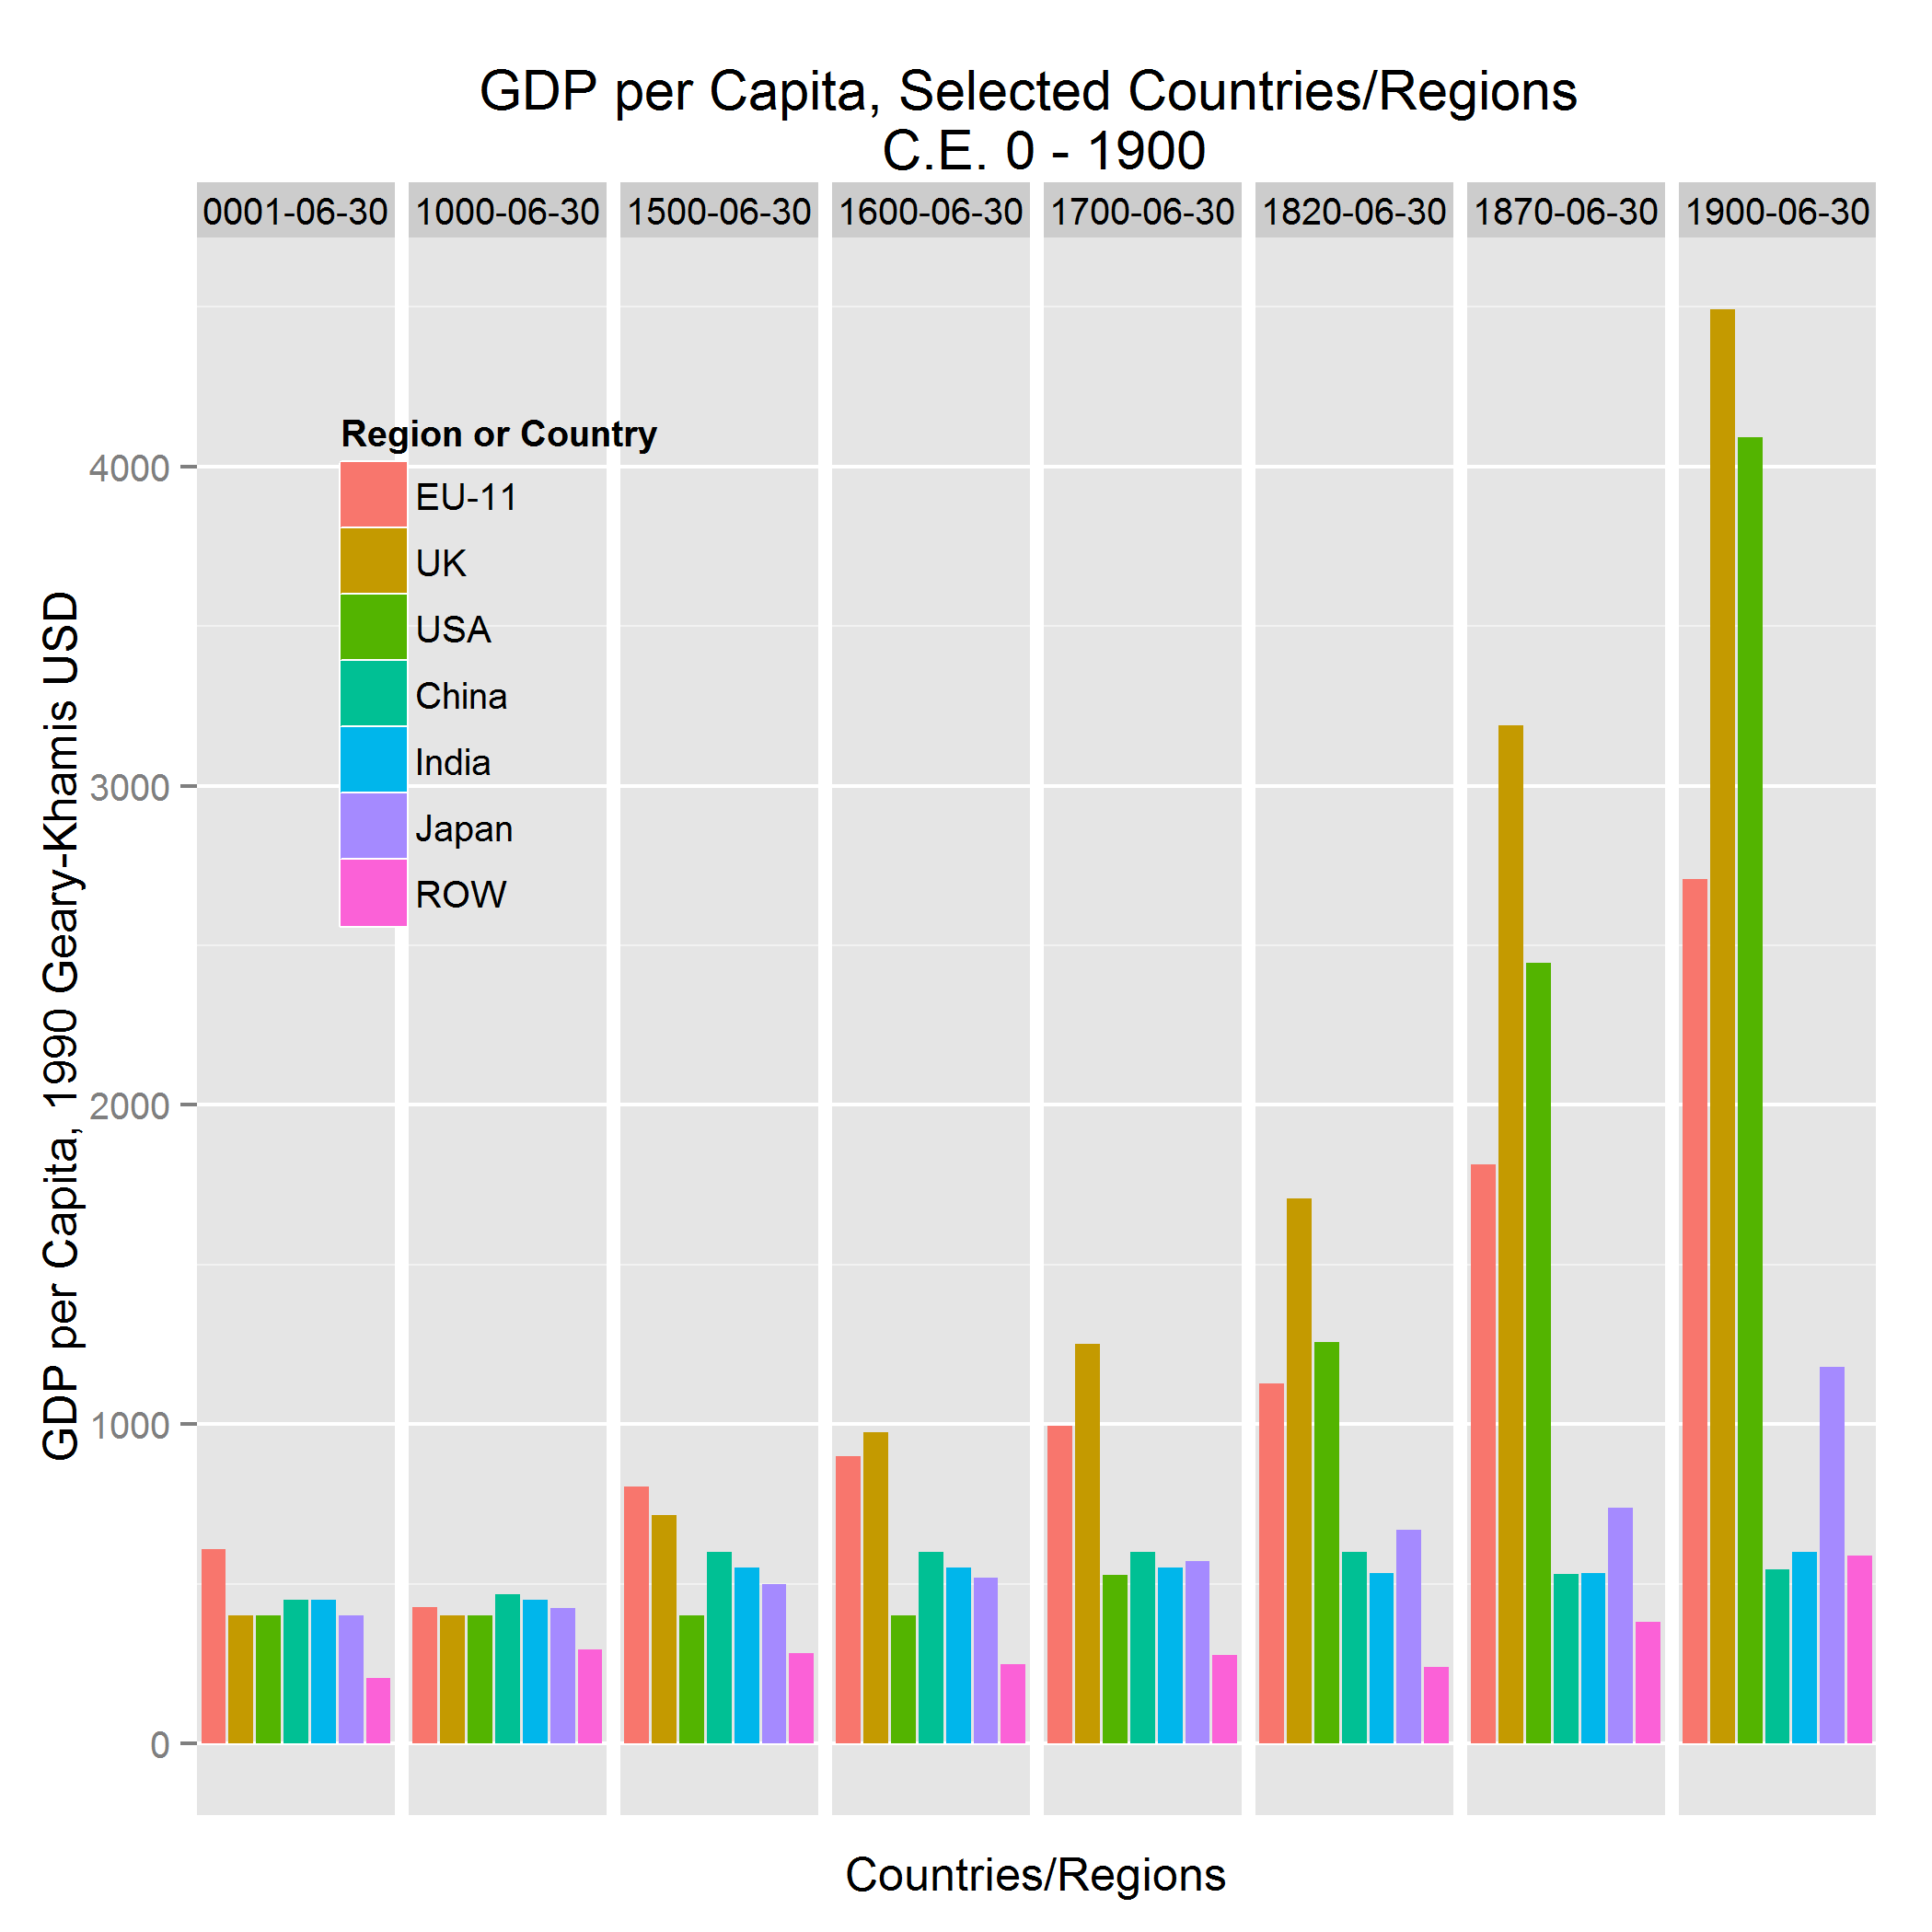
\includegraphics[width=0.8\textwidth]{ggdpcapitadodge.png}
		\caption{Comparative World Per-Capita GDP. \textit{Source:} Data from Maddison (\citeyear{maddison_maddison_2010}), graphs by author.}
		\label{fig:capita}
		\end{figure}
		
		\begin{figure}[htb]
		\centering
		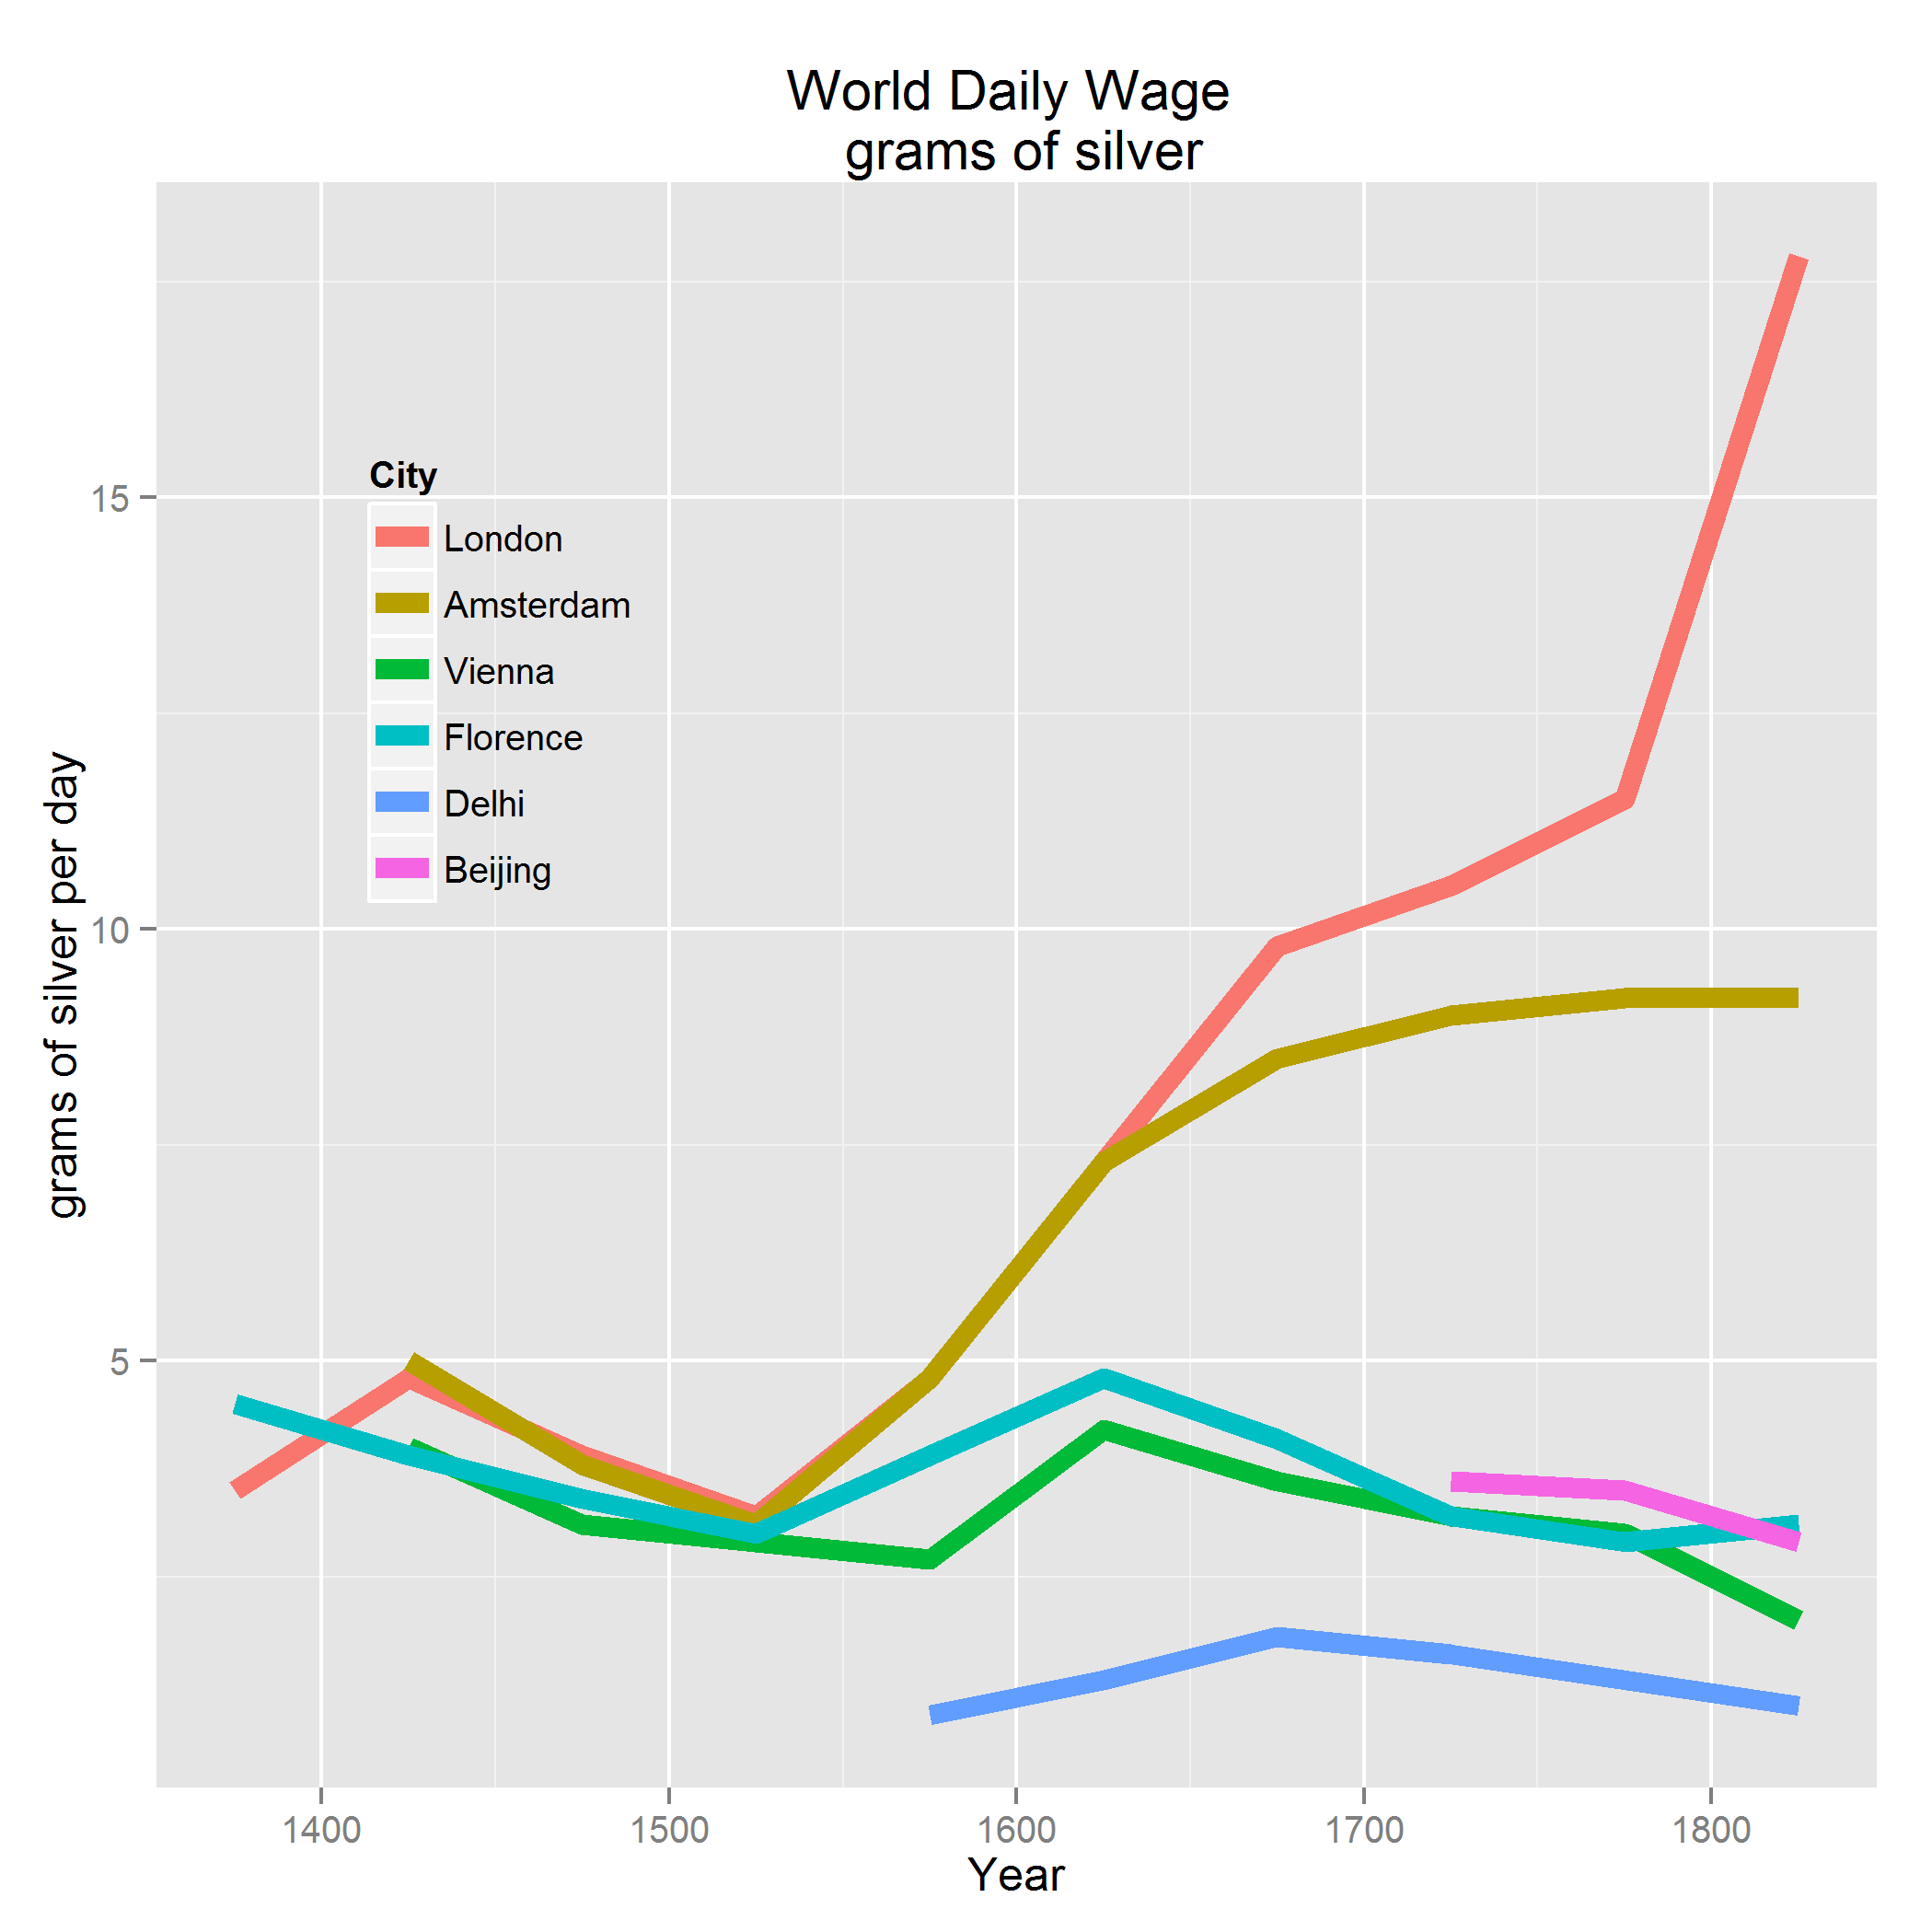
\includegraphics[width=0.9\textwidth]{gworldwages.png} 
		\caption{World wages, CE 1375 -- 1825. \textit{Source:} Allen (\citeyear{allen_british_2009}) \label{fig:allen_wages}}

		\end{figure}
		
		\begin{figure}[htb]
		\centering
		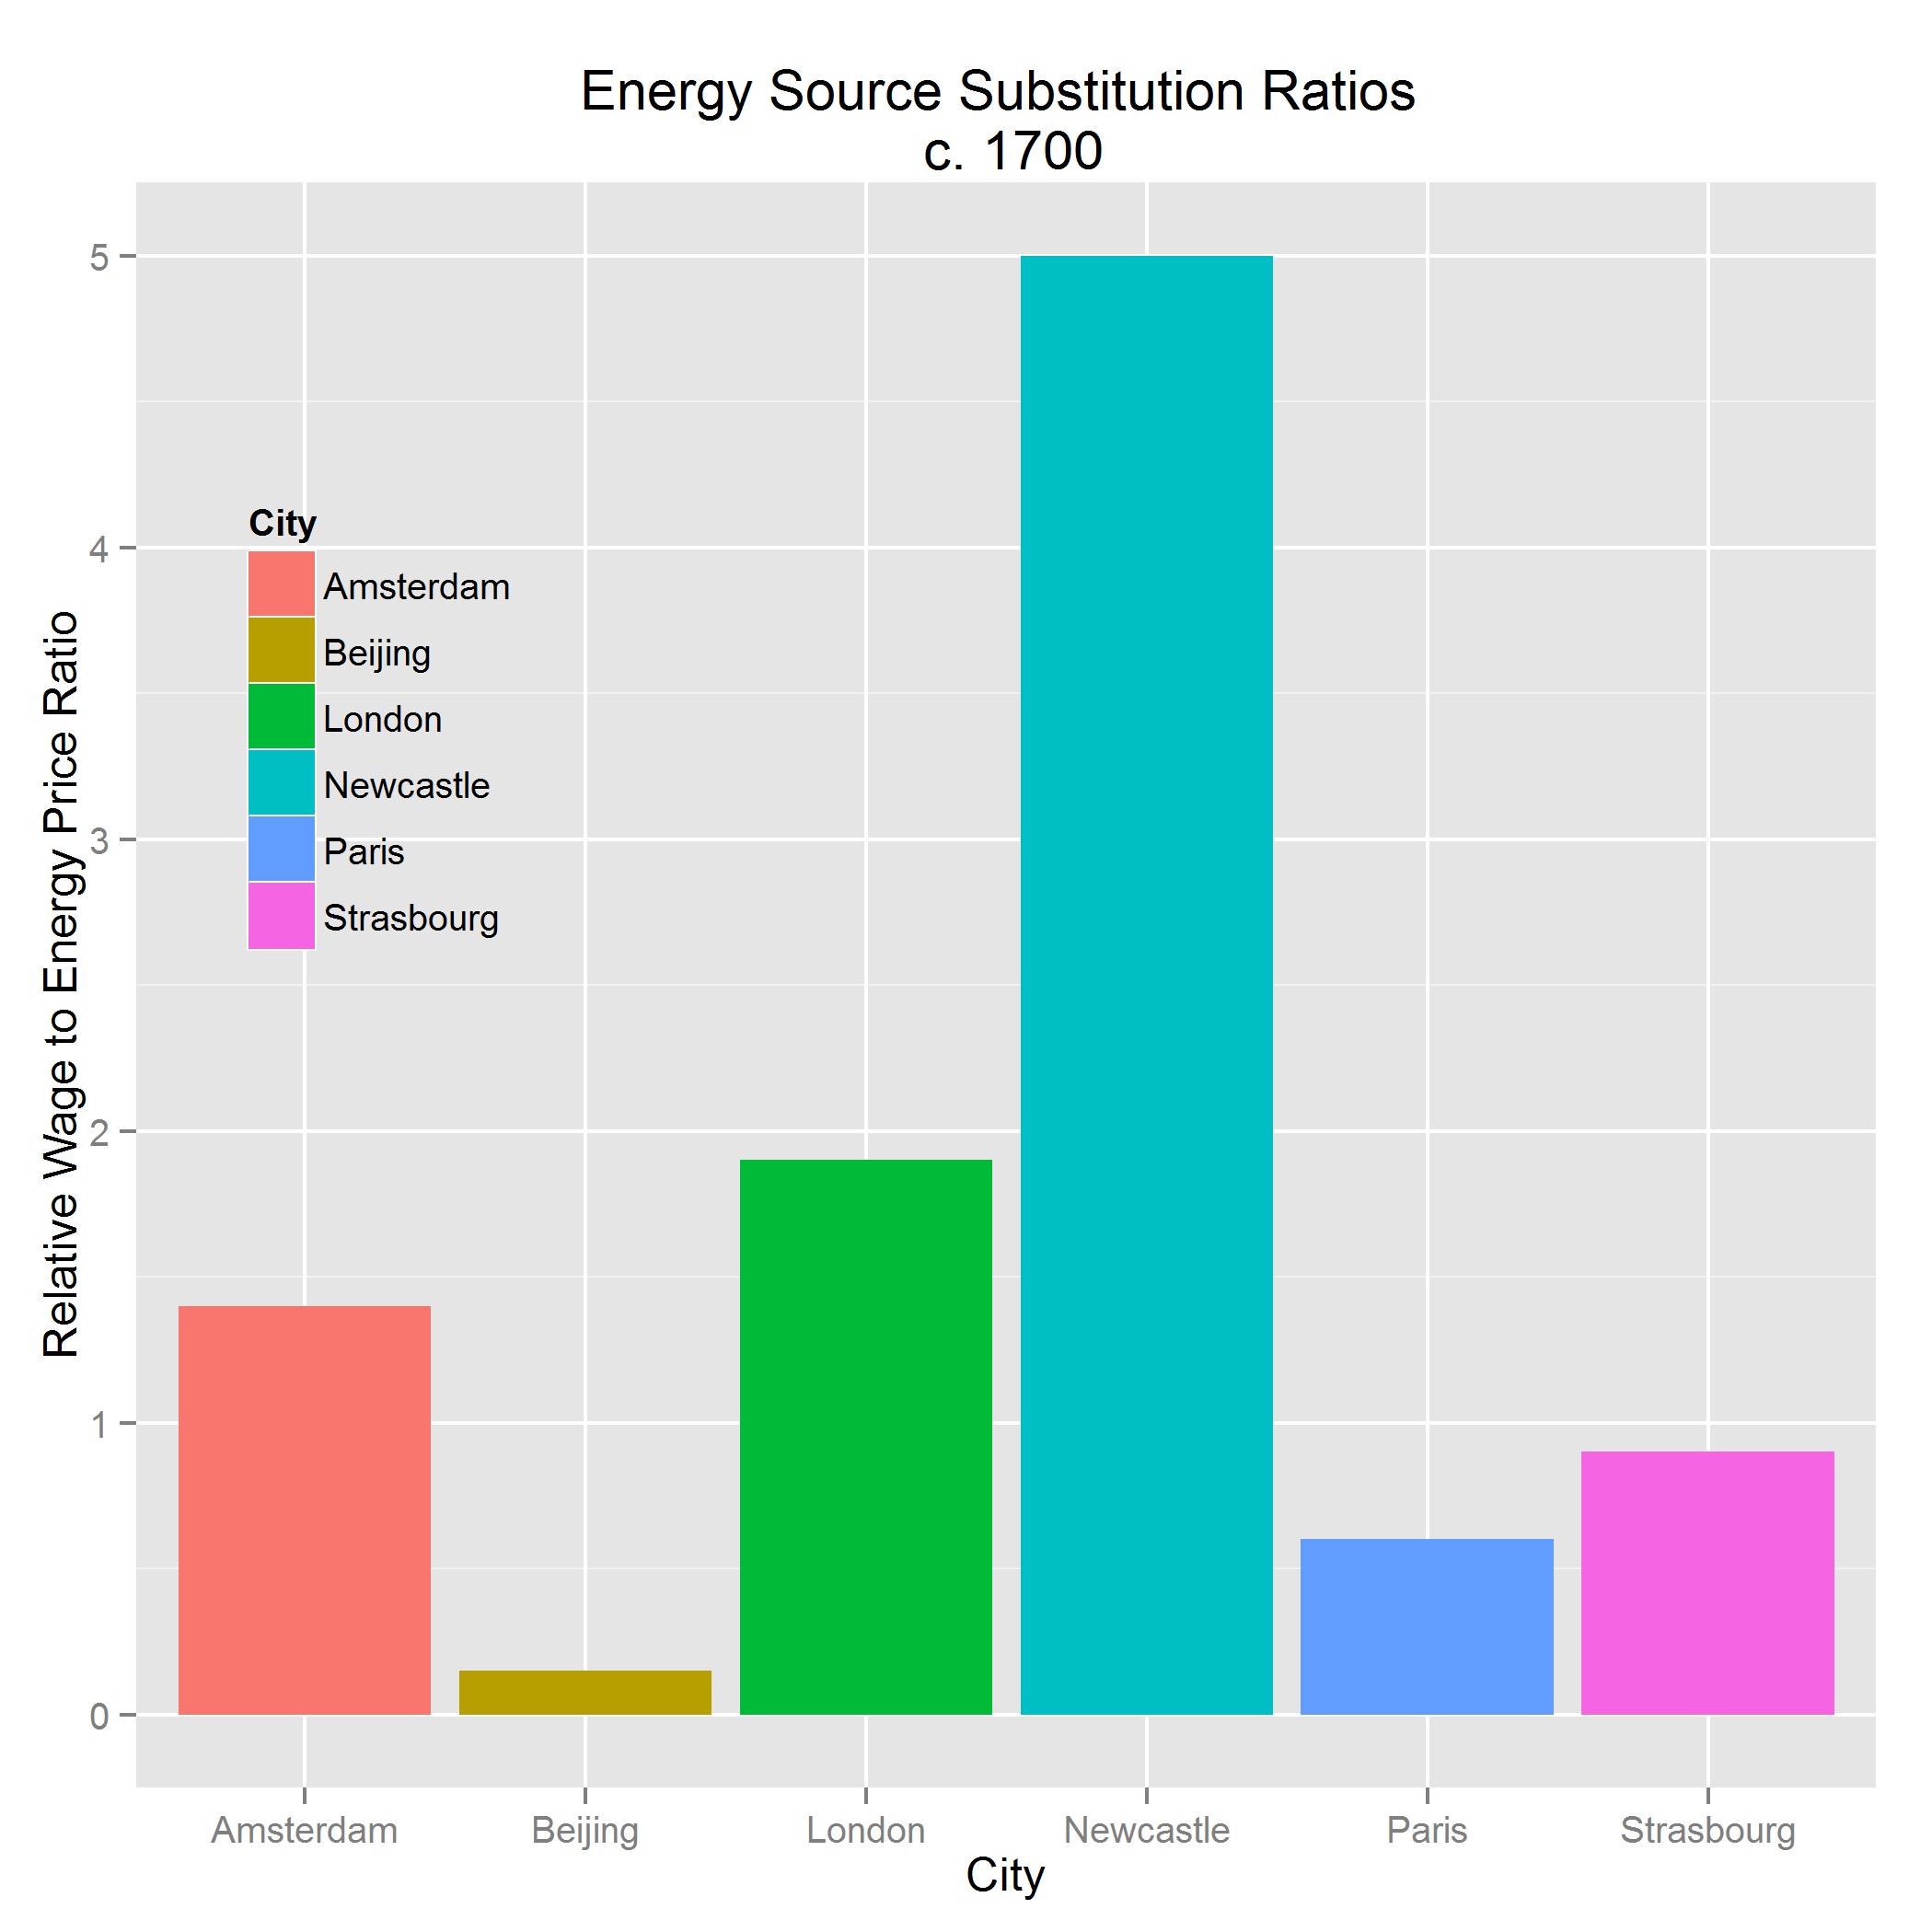
\includegraphics[width=0.8\textwidth]{wage-energy.png}
		\caption{Wage/Energy ratios, 1700 CE. \textit{Source:} Allen (\citeyear{allen_british_2009})}
		\label{fig:allen_ratios}
		\end{figure}
		
		\begin{figure}[htb]
		\centering
		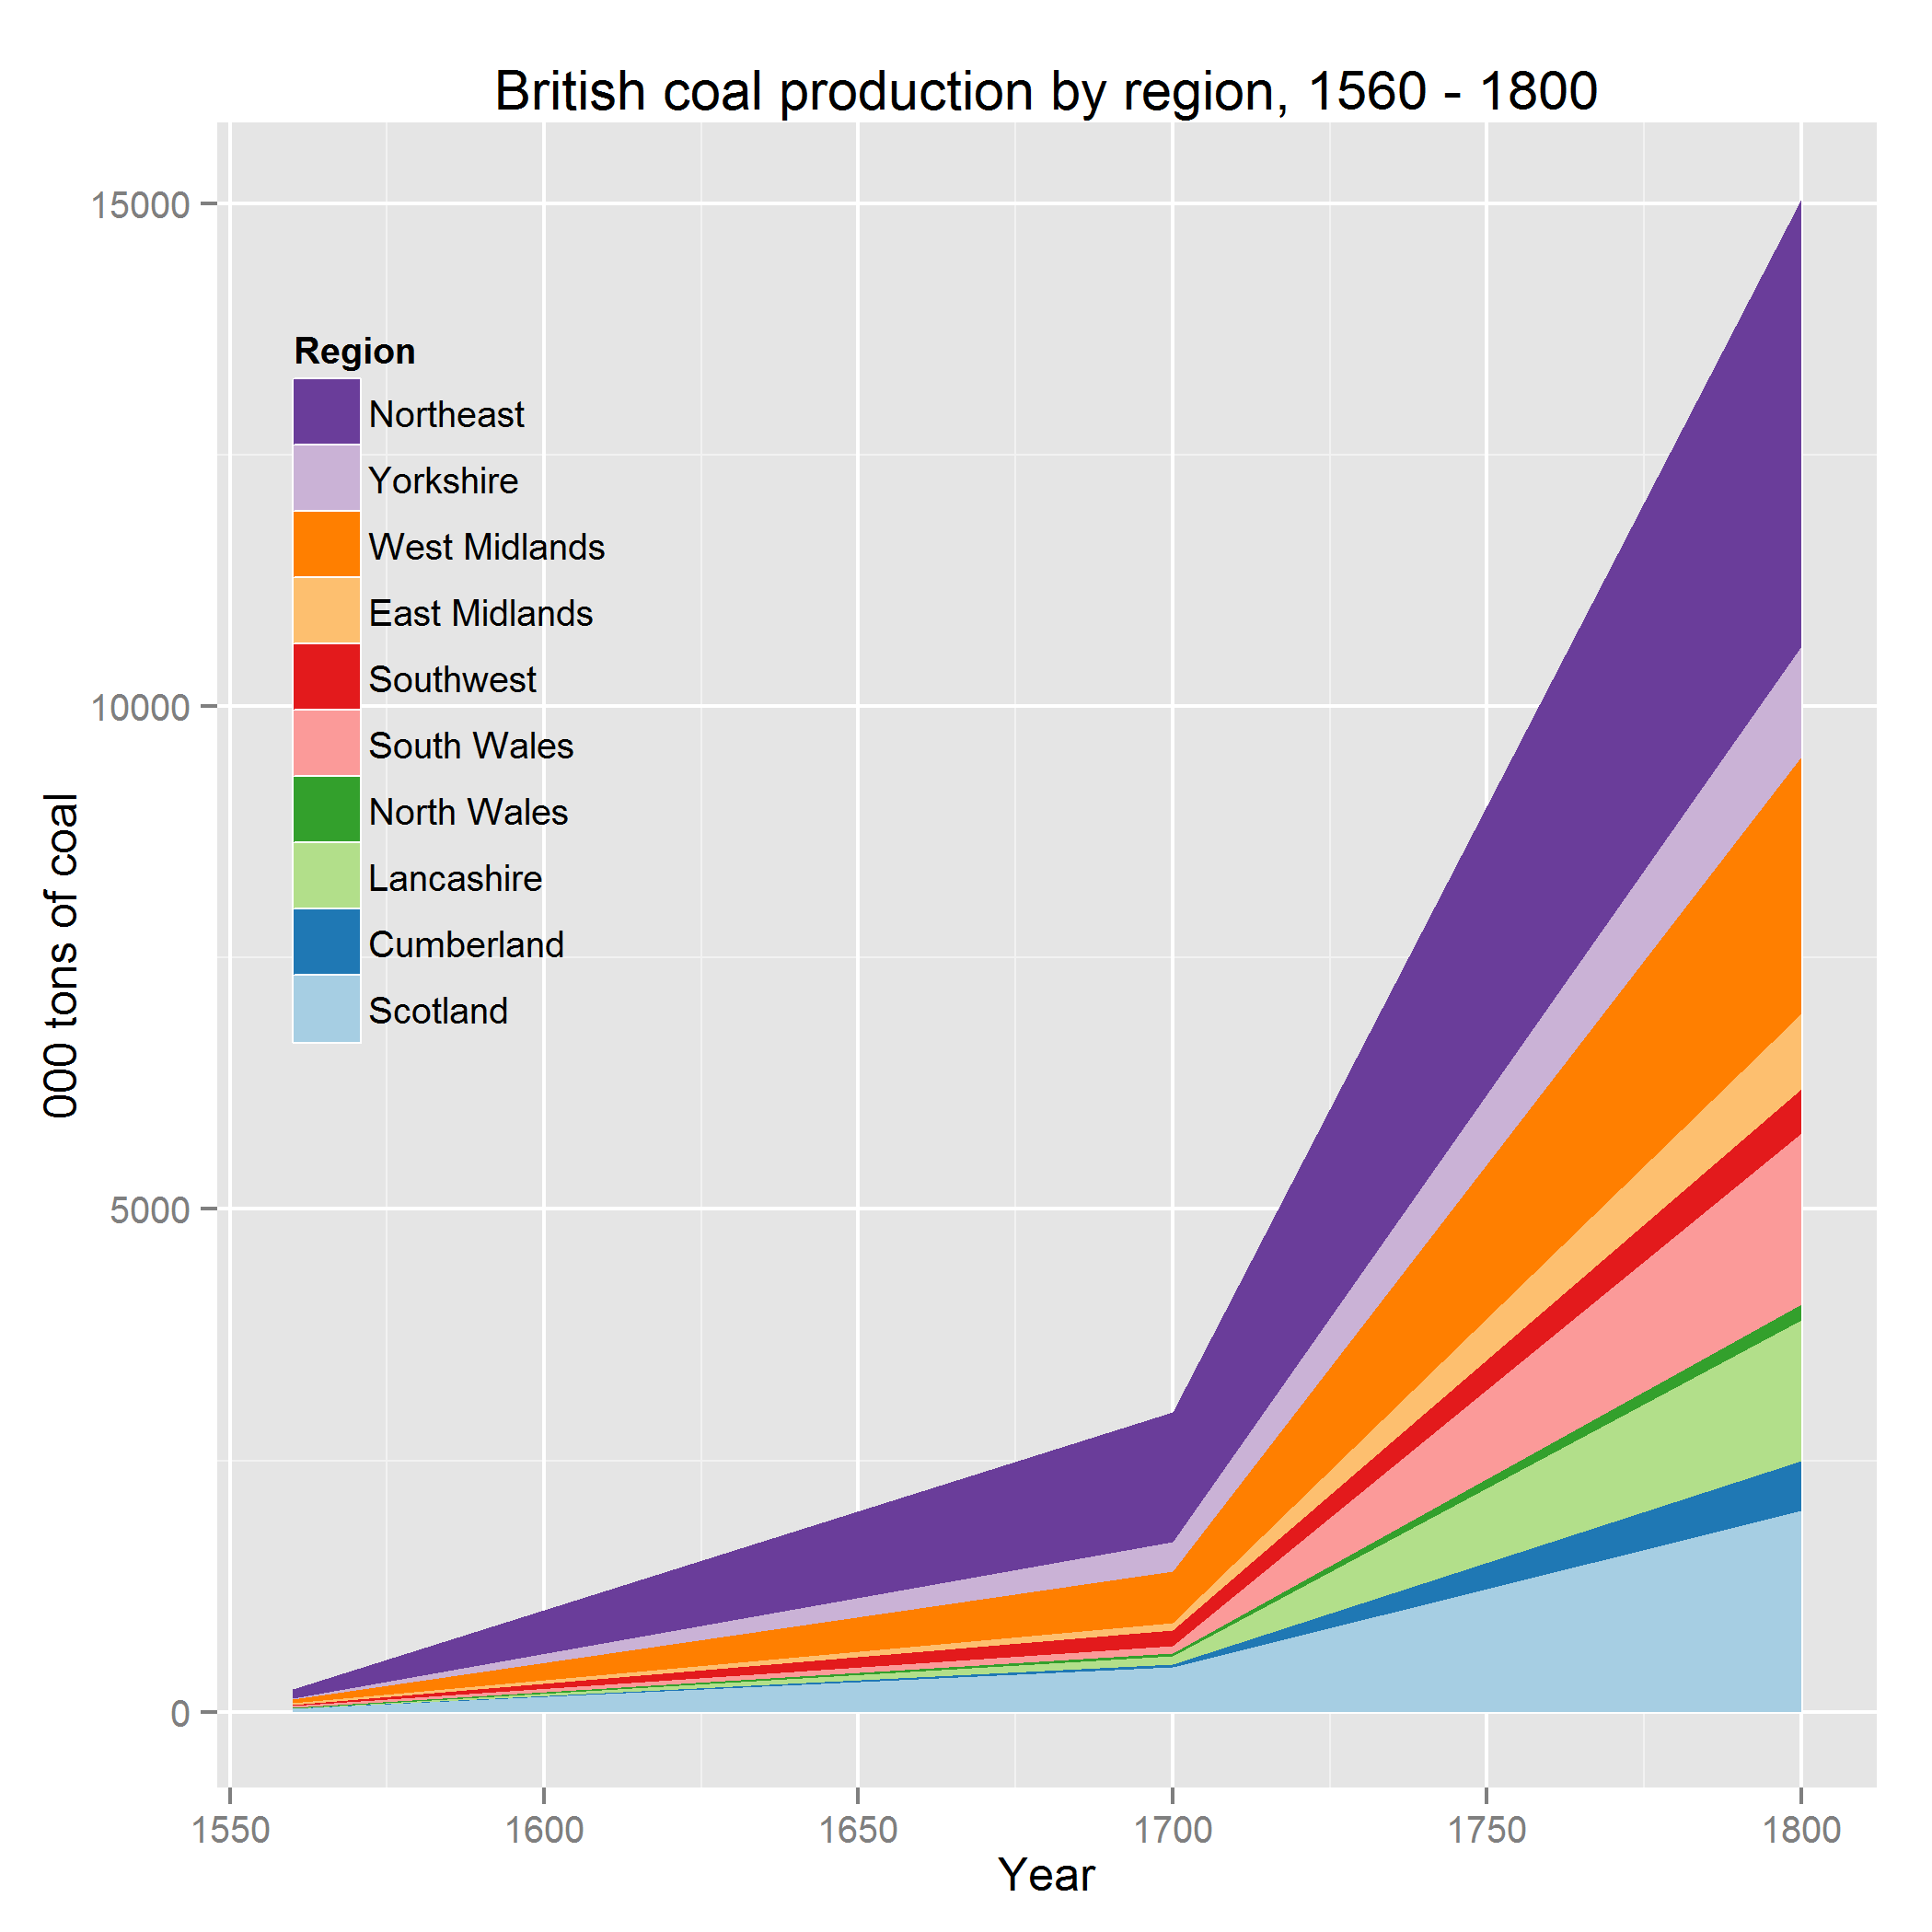
\includegraphics[width=0.8\textwidth]{allen_coal.png}
		\caption{English coal production, CE 1560 -- 1800. \textit{Source:} Allen's data (\citeyear{allen_british_2009}) , graph by author.}
		\label{fig:allen_coal}
		\end{figure}

		\begin{figure}[ftb]
		\centerline{
		\mbox{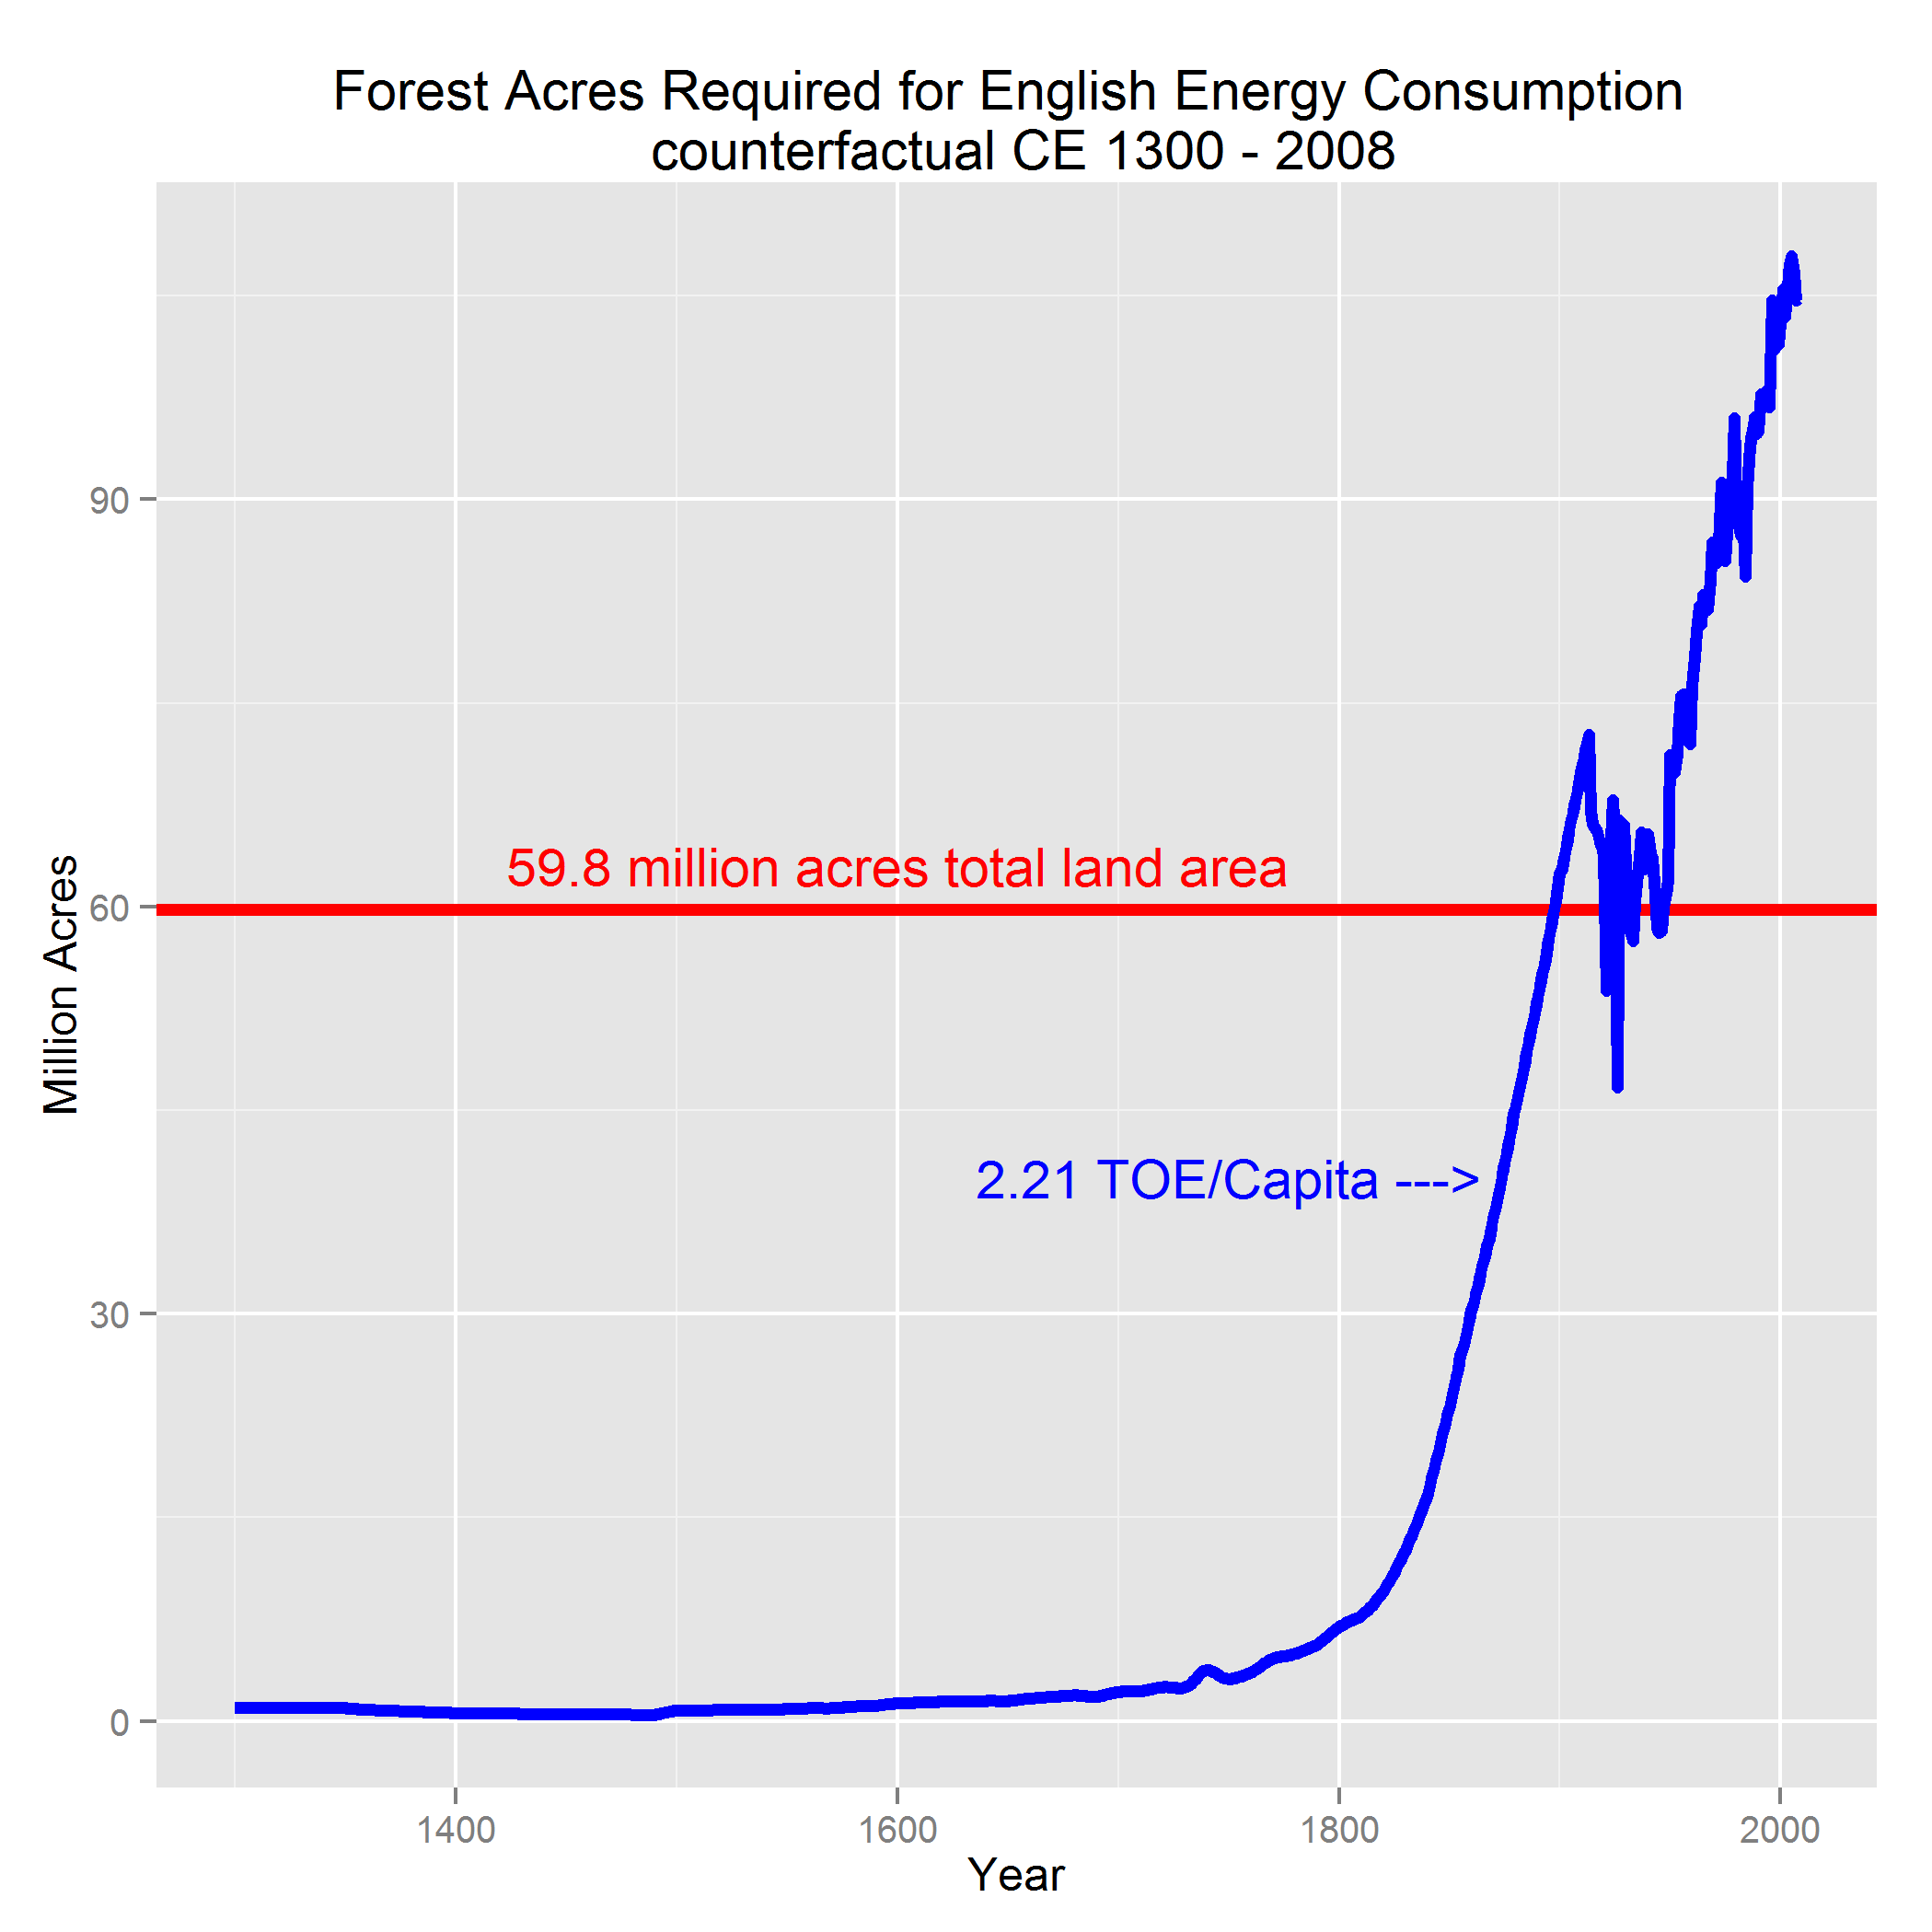
\includegraphics[width=0.70\textwidth]{wood.png}}
		\mbox{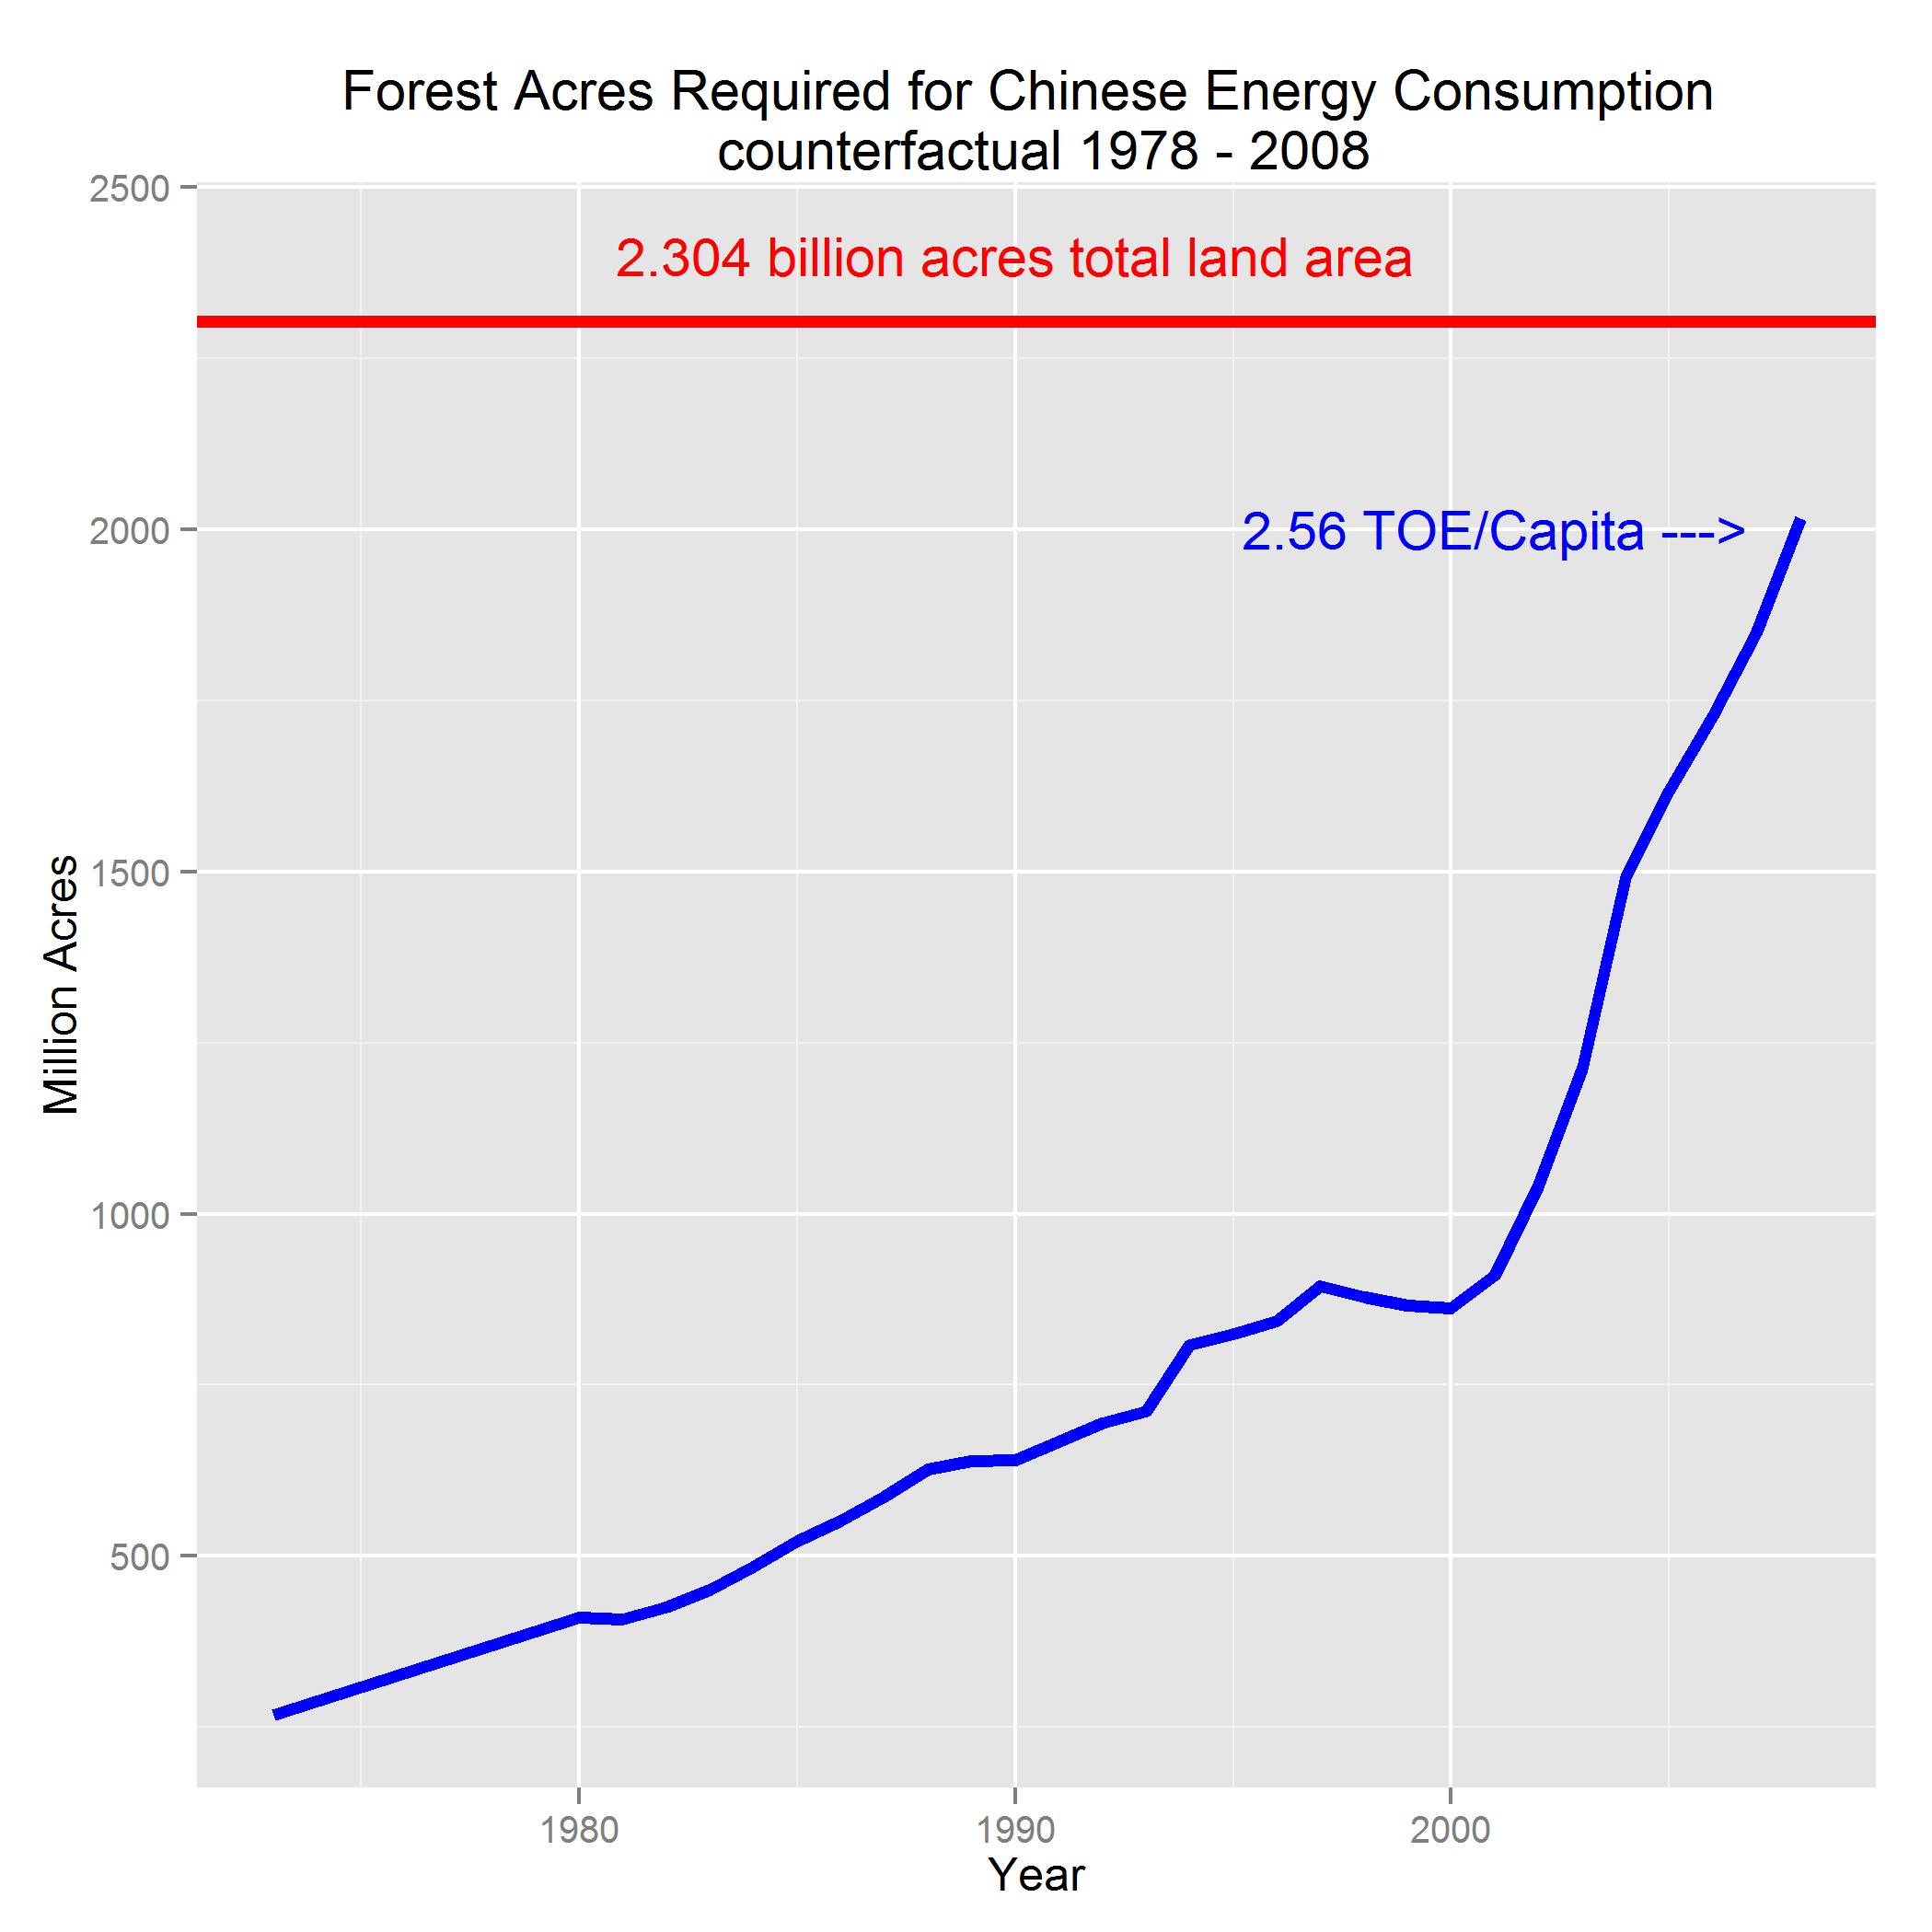
\includegraphics[width=0.70\textwidth]{chinawood.png}}
		}
		\caption{Projected English and Chinese wood fuel requirements. \textit{Source:} Roger Fouquet's energy consumption data (England) (\citeyear{fouquet_heat_2008}), U.S. DOE (China) and the author's calculations.} 
		\label{fig:eng_wood}
		\end{figure}
		

		\begin{figure}[ftb]
		\centering
		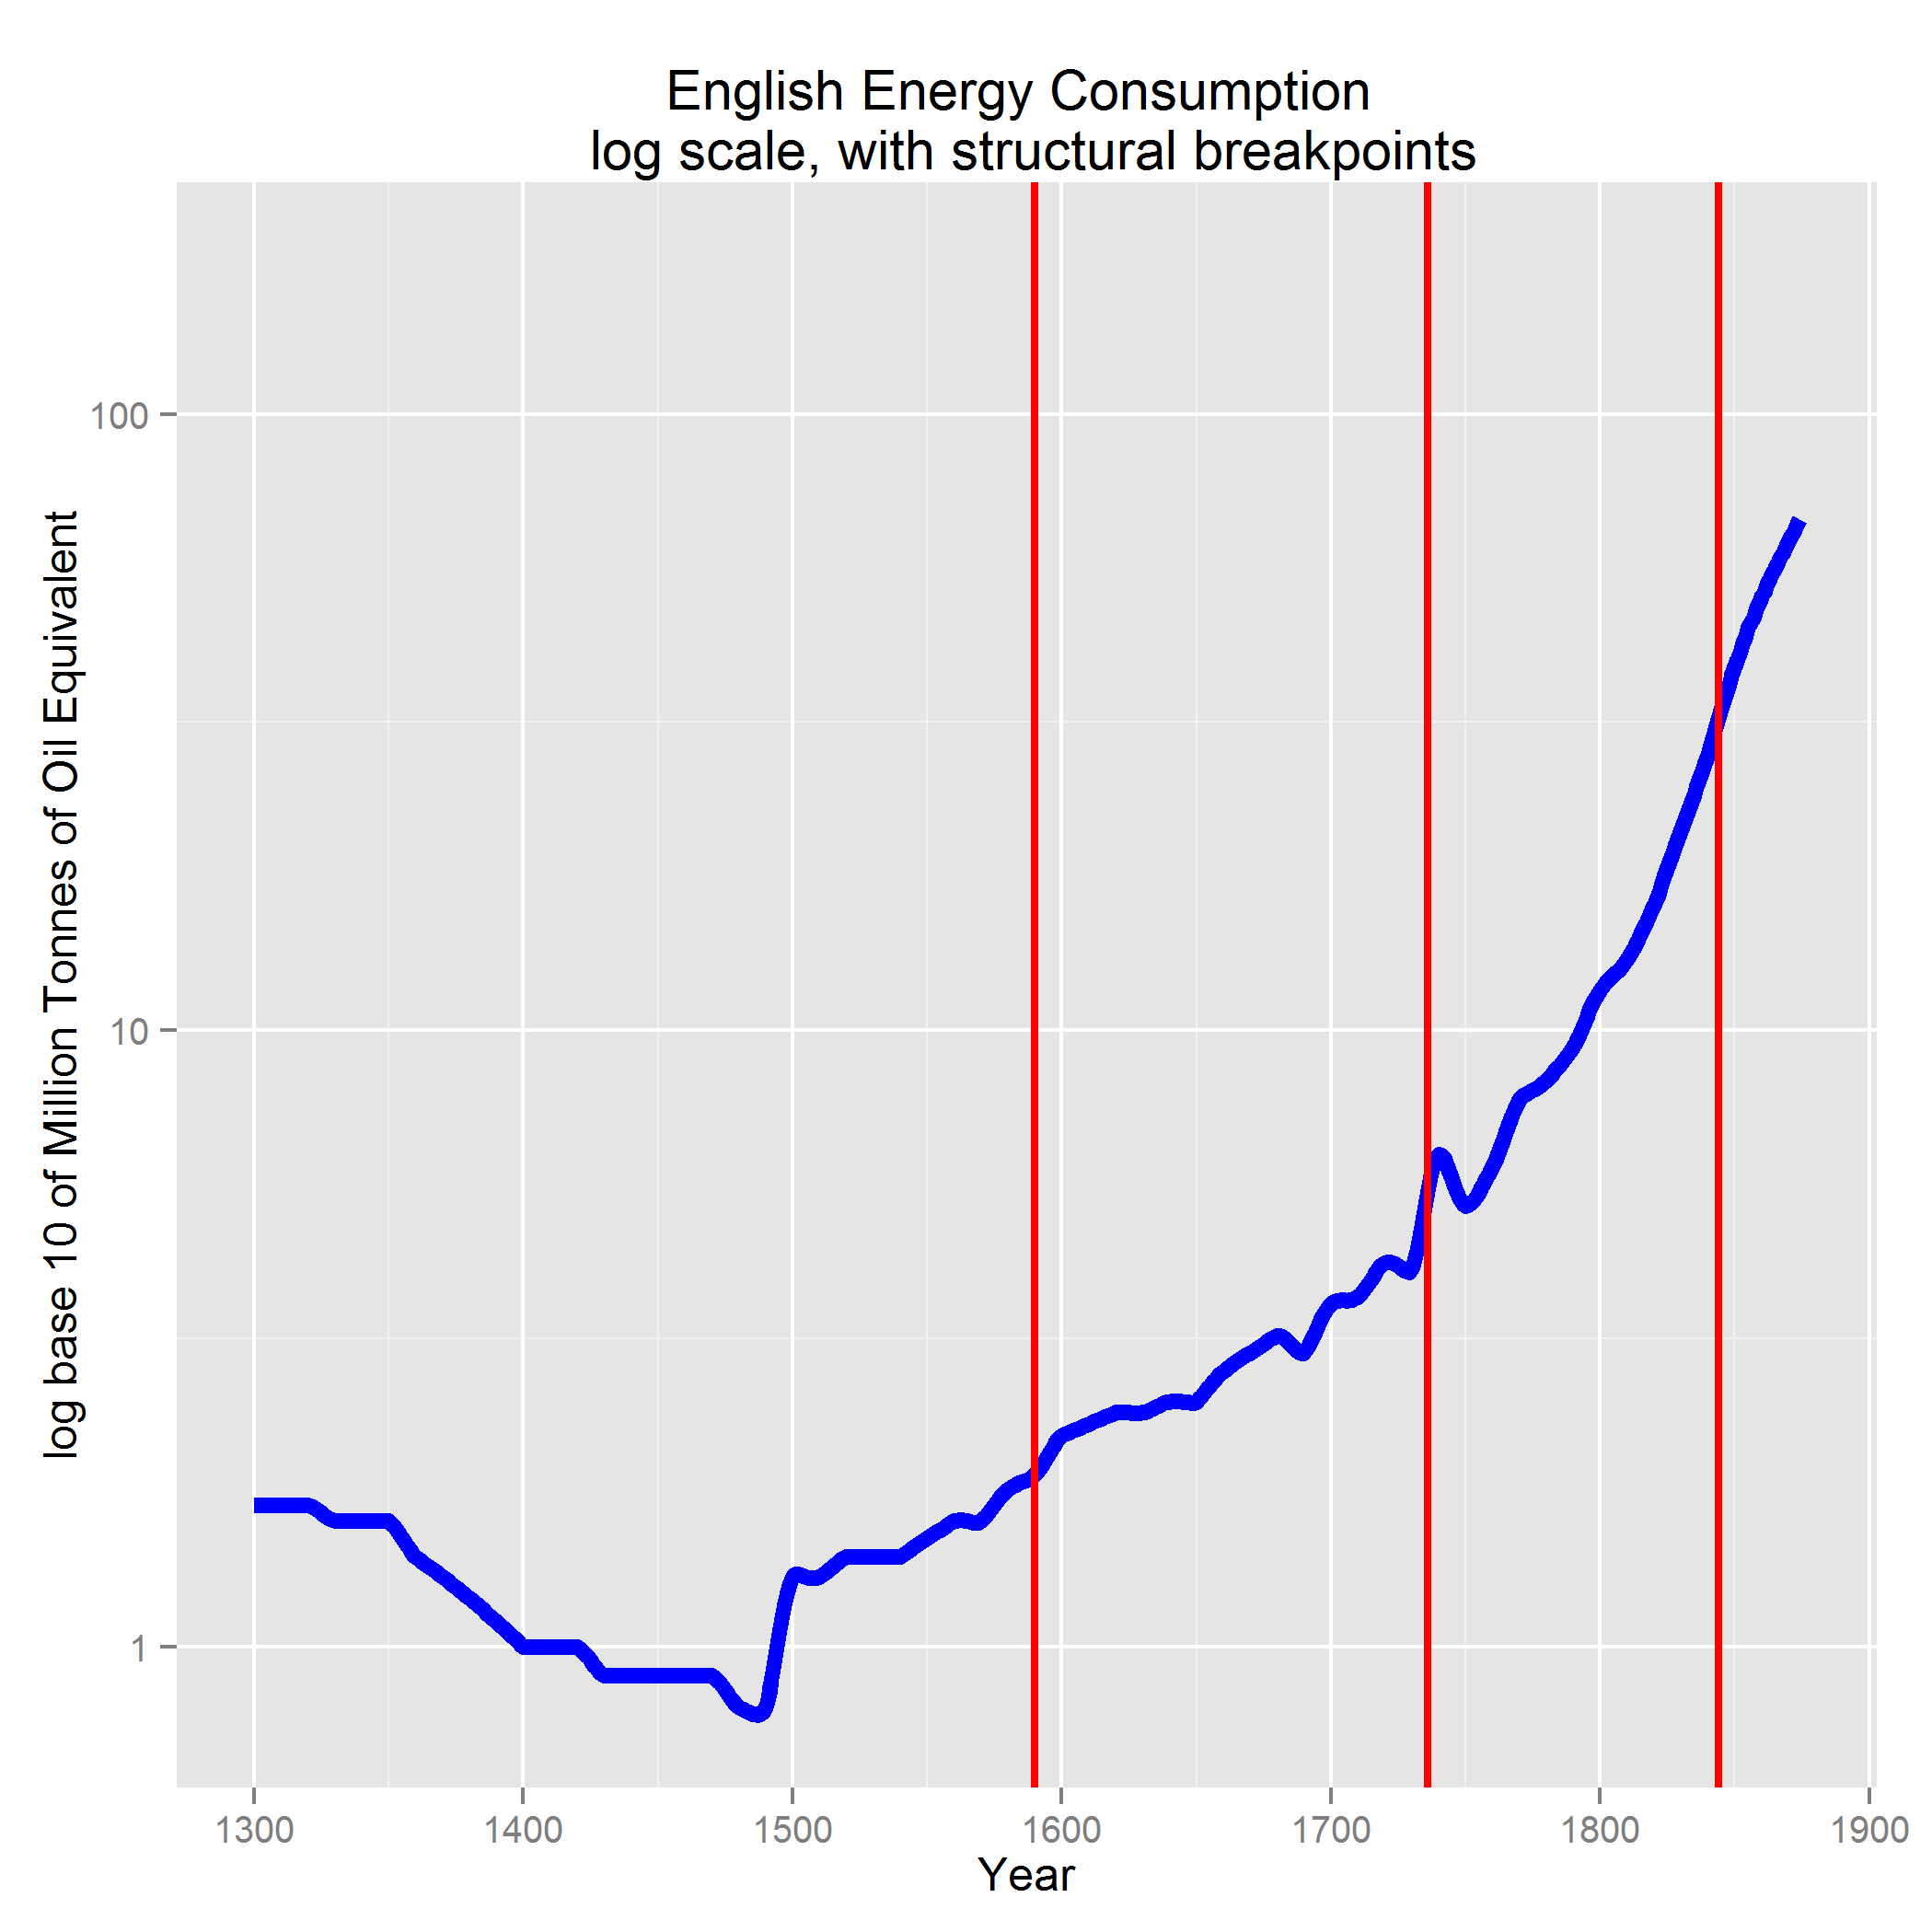
\includegraphics[width=0.8\textwidth]{gbpmtoelog.png}
		\caption{The English Energy Revolution, in logs. \textit{Source:} Roger Fouquet's energy consumption data (\citeyear{fouquet_heat_2008}) and the author's calculations.} 
		\label{fig:mtoe_log}
		\end{figure} 		


\listoffigures

%\section{end of document}
\end{document}



\subsection{sequence for bibliography}

pdflatex
bibtex on .bib
pdflatex
pdflatex
bibtex on .tex
pdflatex
pdflatex

\section{Notes}
11/11/12\\
soften institutional part in intro\\
add in history stuff from SHOE threads\\
in fundamental neoclassical model, note that can also be interpreted  production prices and effective demand, so surplus and distribution\\
ssha inputs

12/25/12
[1] "read.csv(\"maddison.reg.gdp.pct.csv\","
[1] "Settings/Russell/Desktop/VAT/Projects/Research/Conferences/1211ssha/images/maddisonreggdppct.png')"
[1] "read.csv(\"maddison.reg.gdp.csv\","
[1] "Settings/Russell/Desktop/VAT/Projects/Research/Conferences/1211ssha/images/maddisonreggdplevels.png')"
[1] "read.csv(\"maddison.reg.gdp.csv\","
[1] "Settings/Russell/Desktop/VAT/Projects/Research/Conferences/1211ssha/images/maddisonreggdplevels1900.png')"
[1] "read.csv(\"maddison.reg.pop.pct.csv\","
[1] "Settings/Russell/Desktop/VAT/Projects/Research/Conferences/1211ssha/images/maddisonregpoppct.png')"
[1] "read.csv(\"maddison.reg.pop.csv\","
[1] "Settings/Russell/Desktop/VAT/Projects/Research/Conferences/1211ssha/images/maddisonregpoplevels.png')"
[1] "read.csv(\"maddison.reg.pop.csv\","
[1] "Settings/Russell/Desktop/VAT/Projects/Research/Conferences/1211ssha/images/maddisonregpoplevels1900.png')"

> parse <- scan(file='allen_energy.R',what=character())
Read 213 items
> grep('.png',parse)
[1] 170 213
> for(n in grep('.png',parse))print(parse[n])
[1] "Settings/Russell/Desktop/VAT/Projects/Research/Conferences/1204CSBS/images/gworldenergycost.png')"
[1] "Settings/Russell/Desktop/VAT/Projects/Research/Conferences/1204CSBS/images/gworldwages.png')"

> parse <- scan(file='allen_coal.R',what=character())
Read 165 items
> grep('.png',parse)
[1] 119
> for(n in grep('.png',parse))print(parse[n])
[1] "png(\"pics/oneplottime.png\")"

\subsection{image/script/data table}	
\begin{longtable}{lll}
png image&script&data file\\
\hline
maddisonregpoplevels&maddison.gdp.R&maddison.reg.pop.csv\\
maddisonreggdplevles&maddison.gdp.R&maddison.reg.gdp.csv\\
maddisonregpoplevels1900&maddison.gdp.R&maddison.reg.pop.csv\\
maddisonreggdplevels1900&maddiosn.gdp.R&maddison.reg.gdp.csv\\
maddisonregpoppct&maddison.gdp.R&maddison.reg.pop.pct.csv\\
maddisonreggdppct&maddison.gdp.R&maddison.reg.gdp.pct.csv\\
ggdpcapitadodge&gdppop.R&gdp.ex.csv,pop.ex.csv\\
gworldwages&allen\_energy.R&allen\_wages1.csv\\
wage-energy&defense.R&df with ratio,city names\\
allen\_coal&allen\_coal.R&allen\_coal.csv\\
wood&defense.R&gothenburg.Rdata\\
chinawood&defense.R&china.energy.csv\\
gbmtoelog&defense.R&dissert.RData\\
\end{longtable}
